% Options for packages loaded elsewhere
\PassOptionsToPackage{unicode}{hyperref}
\PassOptionsToPackage{hyphens}{url}
%
\documentclass[
  ignorenonframetext,
]{beamer}
\usepackage{pgfpages}
\setbeamertemplate{caption}[numbered]
\setbeamertemplate{caption label separator}{: }
\setbeamercolor{caption name}{fg=normal text.fg}
\beamertemplatenavigationsymbolsempty
% Prevent slide breaks in the middle of a paragraph
\widowpenalties 1 10000
\raggedbottom
\setbeamertemplate{part page}{
  \centering
  \begin{beamercolorbox}[sep=16pt,center]{part title}
    \usebeamerfont{part title}\insertpart\par
  \end{beamercolorbox}
}
\setbeamertemplate{section page}{
  \centering
  \begin{beamercolorbox}[sep=12pt,center]{part title}
    \usebeamerfont{section title}\insertsection\par
  \end{beamercolorbox}
}
\setbeamertemplate{subsection page}{
  \centering
  \begin{beamercolorbox}[sep=8pt,center]{part title}
    \usebeamerfont{subsection title}\insertsubsection\par
  \end{beamercolorbox}
}
\AtBeginPart{
  \frame{\partpage}
}
\AtBeginSection{
  \ifbibliography
  \else
    \frame{\sectionpage}
  \fi
}
\AtBeginSubsection{
  \frame{\subsectionpage}
}
\usepackage{lmodern}
\usepackage{amssymb,amsmath}
\usepackage{ifxetex,ifluatex}
\ifnum 0\ifxetex 1\fi\ifluatex 1\fi=0 % if pdftex
  \usepackage[T1]{fontenc}
  \usepackage[utf8]{inputenc}
  \usepackage{textcomp} % provide euro and other symbols
\else % if luatex or xetex
  \usepackage{unicode-math}
  \defaultfontfeatures{Scale=MatchLowercase}
  \defaultfontfeatures[\rmfamily]{Ligatures=TeX,Scale=1}
\fi
\usetheme[]{PaloAlto}
\usecolortheme{dolphin}
% Use upquote if available, for straight quotes in verbatim environments
\IfFileExists{upquote.sty}{\usepackage{upquote}}{}
\IfFileExists{microtype.sty}{% use microtype if available
  \usepackage[]{microtype}
  \UseMicrotypeSet[protrusion]{basicmath} % disable protrusion for tt fonts
}{}
\makeatletter
\@ifundefined{KOMAClassName}{% if non-KOMA class
  \IfFileExists{parskip.sty}{%
    \usepackage{parskip}
  }{% else
    \setlength{\parindent}{0pt}
    \setlength{\parskip}{6pt plus 2pt minus 1pt}}
}{% if KOMA class
  \KOMAoptions{parskip=half}}
\makeatother
\usepackage{xcolor}
\IfFileExists{xurl.sty}{\usepackage{xurl}}{} % add URL line breaks if available
\IfFileExists{bookmark.sty}{\usepackage{bookmark}}{\usepackage{hyperref}}
\hypersetup{
  pdftitle={Quick high quality maps with R},
  pdfauthor={Jan-Philipp Kolb},
  hidelinks,
  pdfcreator={LaTeX via pandoc}}
\urlstyle{same} % disable monospaced font for URLs
\newif\ifbibliography
\usepackage{color}
\usepackage{fancyvrb}
\newcommand{\VerbBar}{|}
\newcommand{\VERB}{\Verb[commandchars=\\\{\}]}
\DefineVerbatimEnvironment{Highlighting}{Verbatim}{commandchars=\\\{\}}
% Add ',fontsize=\small' for more characters per line
\usepackage{framed}
\definecolor{shadecolor}{RGB}{248,248,248}
\newenvironment{Shaded}{\begin{snugshade}}{\end{snugshade}}
\newcommand{\AlertTok}[1]{\textcolor[rgb]{0.94,0.16,0.16}{#1}}
\newcommand{\AnnotationTok}[1]{\textcolor[rgb]{0.56,0.35,0.01}{\textbf{\textit{#1}}}}
\newcommand{\AttributeTok}[1]{\textcolor[rgb]{0.77,0.63,0.00}{#1}}
\newcommand{\BaseNTok}[1]{\textcolor[rgb]{0.00,0.00,0.81}{#1}}
\newcommand{\BuiltInTok}[1]{#1}
\newcommand{\CharTok}[1]{\textcolor[rgb]{0.31,0.60,0.02}{#1}}
\newcommand{\CommentTok}[1]{\textcolor[rgb]{0.56,0.35,0.01}{\textit{#1}}}
\newcommand{\CommentVarTok}[1]{\textcolor[rgb]{0.56,0.35,0.01}{\textbf{\textit{#1}}}}
\newcommand{\ConstantTok}[1]{\textcolor[rgb]{0.00,0.00,0.00}{#1}}
\newcommand{\ControlFlowTok}[1]{\textcolor[rgb]{0.13,0.29,0.53}{\textbf{#1}}}
\newcommand{\DataTypeTok}[1]{\textcolor[rgb]{0.13,0.29,0.53}{#1}}
\newcommand{\DecValTok}[1]{\textcolor[rgb]{0.00,0.00,0.81}{#1}}
\newcommand{\DocumentationTok}[1]{\textcolor[rgb]{0.56,0.35,0.01}{\textbf{\textit{#1}}}}
\newcommand{\ErrorTok}[1]{\textcolor[rgb]{0.64,0.00,0.00}{\textbf{#1}}}
\newcommand{\ExtensionTok}[1]{#1}
\newcommand{\FloatTok}[1]{\textcolor[rgb]{0.00,0.00,0.81}{#1}}
\newcommand{\FunctionTok}[1]{\textcolor[rgb]{0.00,0.00,0.00}{#1}}
\newcommand{\ImportTok}[1]{#1}
\newcommand{\InformationTok}[1]{\textcolor[rgb]{0.56,0.35,0.01}{\textbf{\textit{#1}}}}
\newcommand{\KeywordTok}[1]{\textcolor[rgb]{0.13,0.29,0.53}{\textbf{#1}}}
\newcommand{\NormalTok}[1]{#1}
\newcommand{\OperatorTok}[1]{\textcolor[rgb]{0.81,0.36,0.00}{\textbf{#1}}}
\newcommand{\OtherTok}[1]{\textcolor[rgb]{0.56,0.35,0.01}{#1}}
\newcommand{\PreprocessorTok}[1]{\textcolor[rgb]{0.56,0.35,0.01}{\textit{#1}}}
\newcommand{\RegionMarkerTok}[1]{#1}
\newcommand{\SpecialCharTok}[1]{\textcolor[rgb]{0.00,0.00,0.00}{#1}}
\newcommand{\SpecialStringTok}[1]{\textcolor[rgb]{0.31,0.60,0.02}{#1}}
\newcommand{\StringTok}[1]{\textcolor[rgb]{0.31,0.60,0.02}{#1}}
\newcommand{\VariableTok}[1]{\textcolor[rgb]{0.00,0.00,0.00}{#1}}
\newcommand{\VerbatimStringTok}[1]{\textcolor[rgb]{0.31,0.60,0.02}{#1}}
\newcommand{\WarningTok}[1]{\textcolor[rgb]{0.56,0.35,0.01}{\textbf{\textit{#1}}}}
\usepackage{graphicx}
\makeatletter
\def\maxwidth{\ifdim\Gin@nat@width>\linewidth\linewidth\else\Gin@nat@width\fi}
\def\maxheight{\ifdim\Gin@nat@height>\textheight\textheight\else\Gin@nat@height\fi}
\makeatother
% Scale images if necessary, so that they will not overflow the page
% margins by default, and it is still possible to overwrite the defaults
% using explicit options in \includegraphics[width, height, ...]{}
\setkeys{Gin}{width=\maxwidth,height=\maxheight,keepaspectratio}
% Set default figure placement to htbp
\makeatletter
\def\fps@figure{htbp}
\makeatother
\setlength{\emergencystretch}{3em} % prevent overfull lines
\providecommand{\tightlist}{%
  \setlength{\itemsep}{0pt}\setlength{\parskip}{0pt}}
\setcounter{secnumdepth}{-\maxdimen} % remove section numbering

\title{Quick high quality maps with R}
\author{Jan-Philipp Kolb}
\date{23 6 2021}

\begin{document}
\frame{\titlepage}

\begin{frame}{Preliminaries}
\protect\hypertarget{preliminaries}{}
\begin{itemize}
\tightlist
\item
  Usually I have big differences in knowledge and abilities of the
  participants - please tell, if it is too fast or slow.
\item
  I have lots of hands-on coding
  \href{http://web.math.ku.dk/~helle/R-intro/exercises.pdf}{\textbf{exercises}}
  - later you can only learn on your own
\item
  We have many \href{https://www.showmeshiny.com/}{\textbf{examples}} -
  try them
\item
  If there are questions - always ask
\item
  R is more fun together - strong proponent of collaborative work!
\end{itemize}
\end{frame}

\begin{frame}{Adjustments for online course}
\protect\hypertarget{adjustments-for-online-course}{}
\begin{itemize}
\tightlist
\item
  Quick
\item
  One slide - one example -
\item
  Easy to use
\end{itemize}
\end{frame}

\begin{frame}[fragile]{Getting help on packages}
\protect\hypertarget{getting-help-on-packages}{}
\begin{Shaded}
\begin{Highlighting}[]
\CommentTok{\# provides details regarding contents of a package}
\KeywordTok{help}\NormalTok{(}\DataTypeTok{package =} \StringTok{"osmplotr"}\NormalTok{)}
\CommentTok{\# list vignettes available for a specific package}
\KeywordTok{vignette}\NormalTok{(}\DataTypeTok{package=}\StringTok{"osmplotr"}\NormalTok{)}
\CommentTok{\# view specific vignette}
\KeywordTok{vignette}\NormalTok{(}\StringTok{"data{-}maps"}\NormalTok{)}
\end{Highlighting}
\end{Shaded}
\end{frame}

\begin{frame}[fragile]{The \texttt{World} dataset}
\protect\hypertarget{the-world-dataset}{}
\begin{block}{Natural Earth}
\protect\hypertarget{natural-earth}{}
\begin{itemize}
\tightlist
\item
  Dataset contains information from
  \href{http://www.naturalearthdata.com/}{\textbf{Natural Earth}}
\end{itemize}

\begin{Shaded}
\begin{Highlighting}[]
\KeywordTok{library}\NormalTok{(tmap)}
\KeywordTok{data}\NormalTok{(World)}
\end{Highlighting}
\end{Shaded}

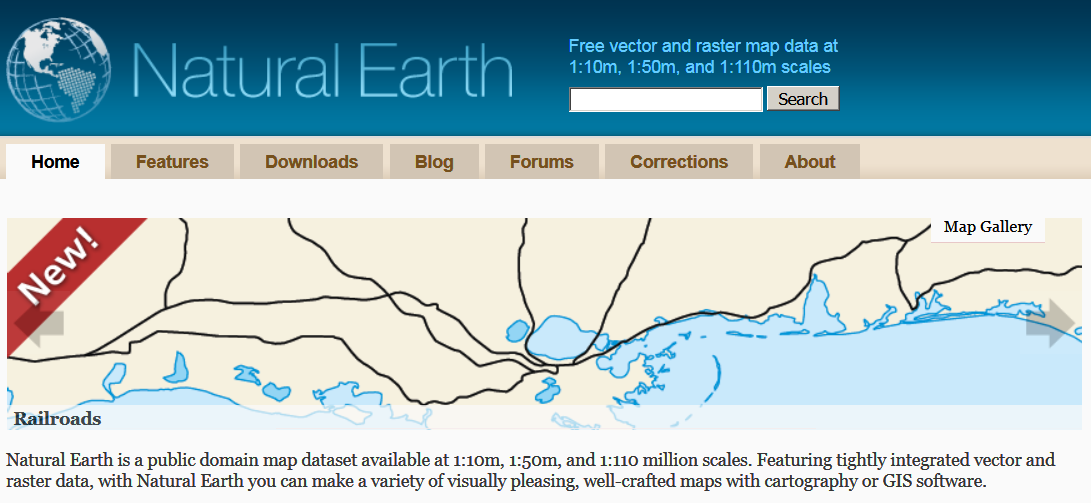
\includegraphics{pics/NaturalEarthData.PNG}
\end{block}
\end{frame}

\begin{frame}[fragile]{The \texttt{qtm} command from the \texttt{tmap}
package}
\protect\hypertarget{the-qtm-command-from-the-tmap-package}{}
\begin{block}{Fast thematic map}
\protect\hypertarget{fast-thematic-map}{}
\begin{itemize}
\item
  With
  \href{https://cran.r-project.org/web/packages/tmap/vignettes/tmap-nutshell.html}{\textbf{qtm}}
  you can create a fast thematic map
\item
  Example from the
  \href{https://cran.r-project.org/web/packages/tmap/vignettes/tmap-nutshell.html}{\textbf{Vignette}}
  for the \texttt{tmap} package
\end{itemize}

\begin{Shaded}
\begin{Highlighting}[]
\KeywordTok{library}\NormalTok{(tmap)}
\KeywordTok{data}\NormalTok{(World)}
\KeywordTok{qtm}\NormalTok{(World)}
\end{Highlighting}
\end{Shaded}

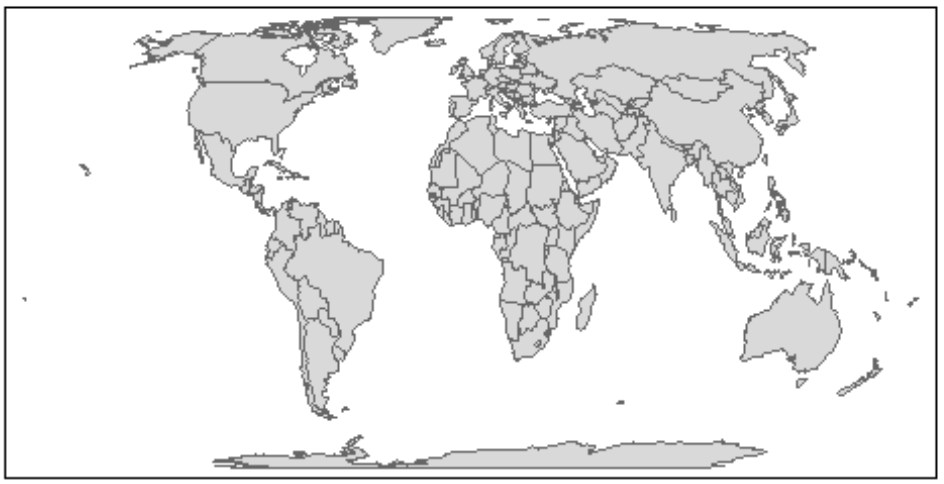
\includegraphics[width=0.5\textwidth,height=\textheight]{pics/qtm_world2.PNG}
\end{block}
\end{frame}

\begin{frame}[fragile]{To get more color in the map}
\protect\hypertarget{to-get-more-color-in-the-map}{}
\begin{block}{Economic development status}
\protect\hypertarget{economic-development-status}{}
\begin{Shaded}
\begin{Highlighting}[]
\KeywordTok{qtm}\NormalTok{(World, }\DataTypeTok{fill=}\StringTok{"economy"}\NormalTok{)}
\end{Highlighting}
\end{Shaded}

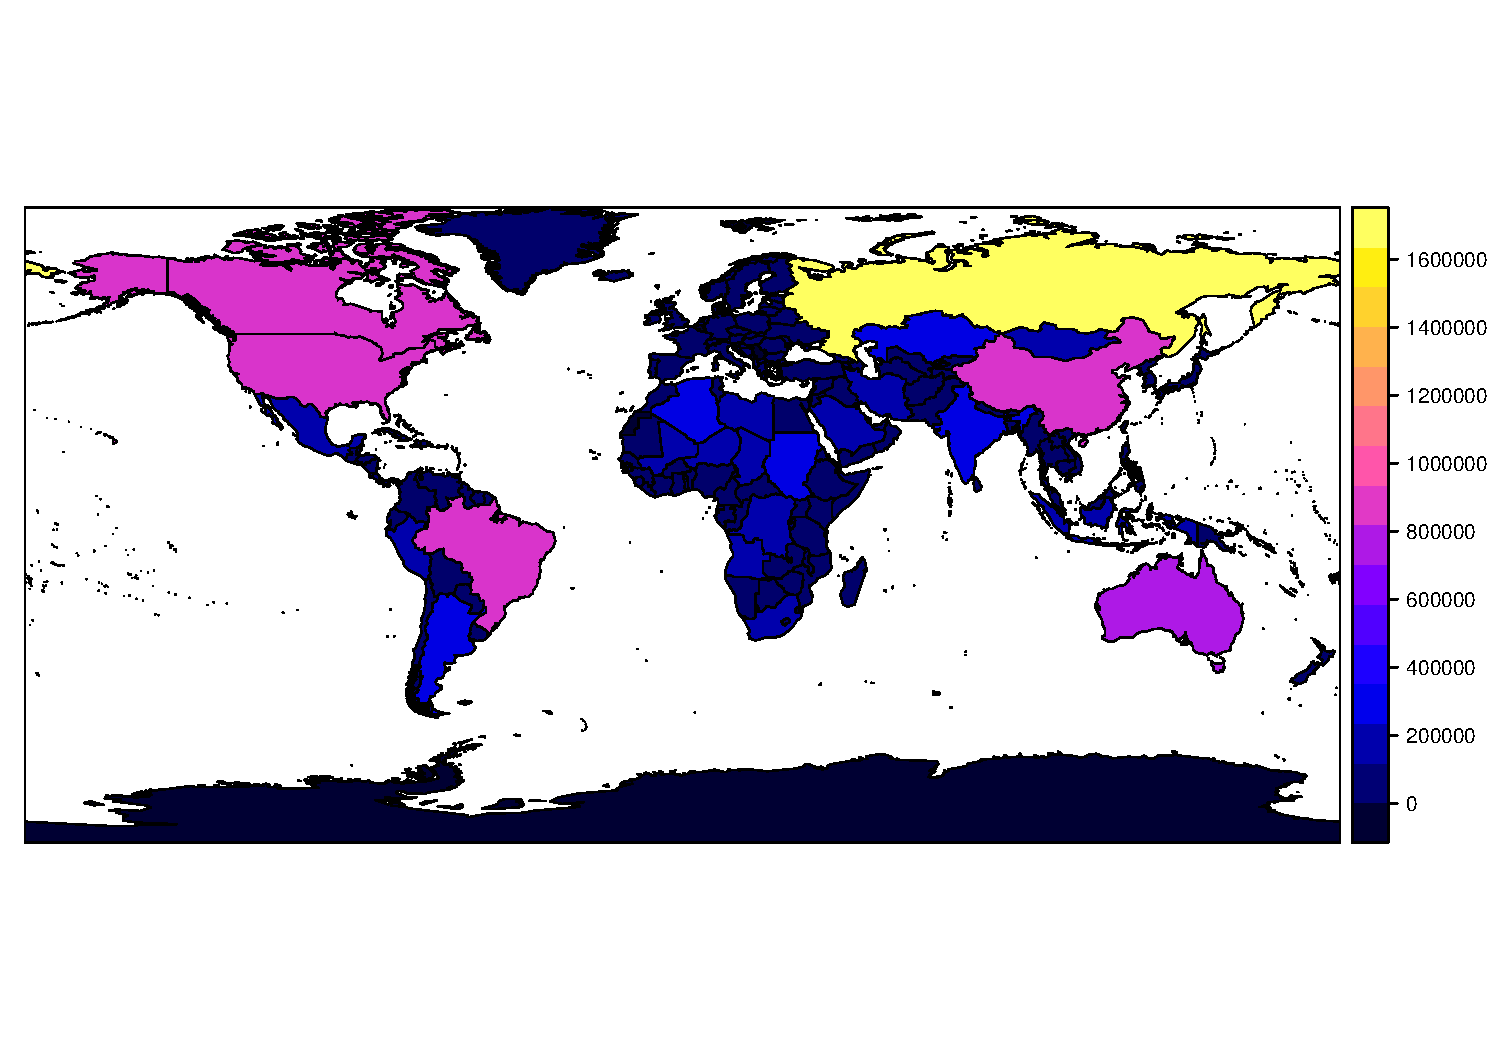
\includegraphics{quick_high_quality_maps_files/figure-beamer/unnamed-chunk-4-1.pdf}
\end{block}
\end{frame}

\begin{frame}[fragile]{A map with text}
\protect\hypertarget{a-map-with-text}{}
\begin{block}{Population}
\protect\hypertarget{population}{}
\begin{Shaded}
\begin{Highlighting}[]
\KeywordTok{qtm}\NormalTok{(World, }\DataTypeTok{fill=}\StringTok{"pop\_est"}\NormalTok{, }\DataTypeTok{text=}\StringTok{"iso\_a3"}\NormalTok{)}
\end{Highlighting}
\end{Shaded}

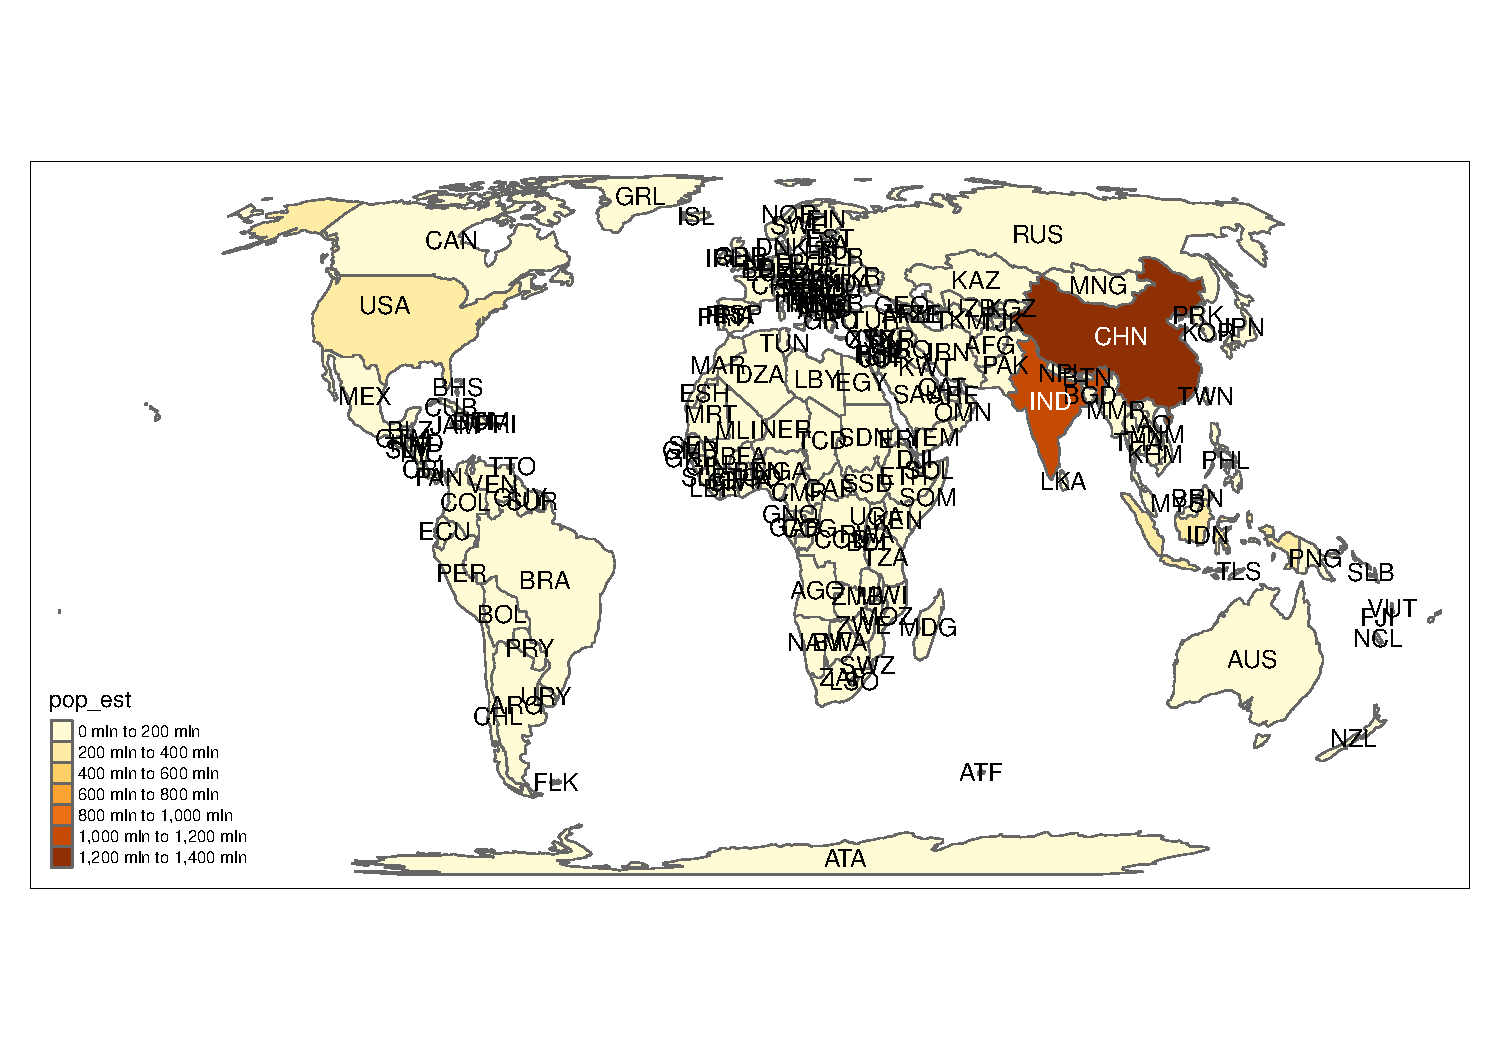
\includegraphics{quick_high_quality_maps_files/figure-beamer/unnamed-chunk-5-1.pdf}
\end{block}
\end{frame}

\begin{frame}[fragile]{This Scheme is better:}
\protect\hypertarget{this-scheme-is-better}{}
\begin{block}{\href{https://en.wikipedia.org/wiki/Population_density}{\textbf{GDP
per capita}}}
\protect\hypertarget{gdp-per-capita}{}
\begin{Shaded}
\begin{Highlighting}[]
\KeywordTok{qtm}\NormalTok{(World, }\DataTypeTok{fill=}\StringTok{"gdp\_cap\_est"}\NormalTok{, }\DataTypeTok{text=}\StringTok{"iso\_a3"}\NormalTok{, }
    \DataTypeTok{text.size=}\StringTok{"AREA"}\NormalTok{)}
\end{Highlighting}
\end{Shaded}

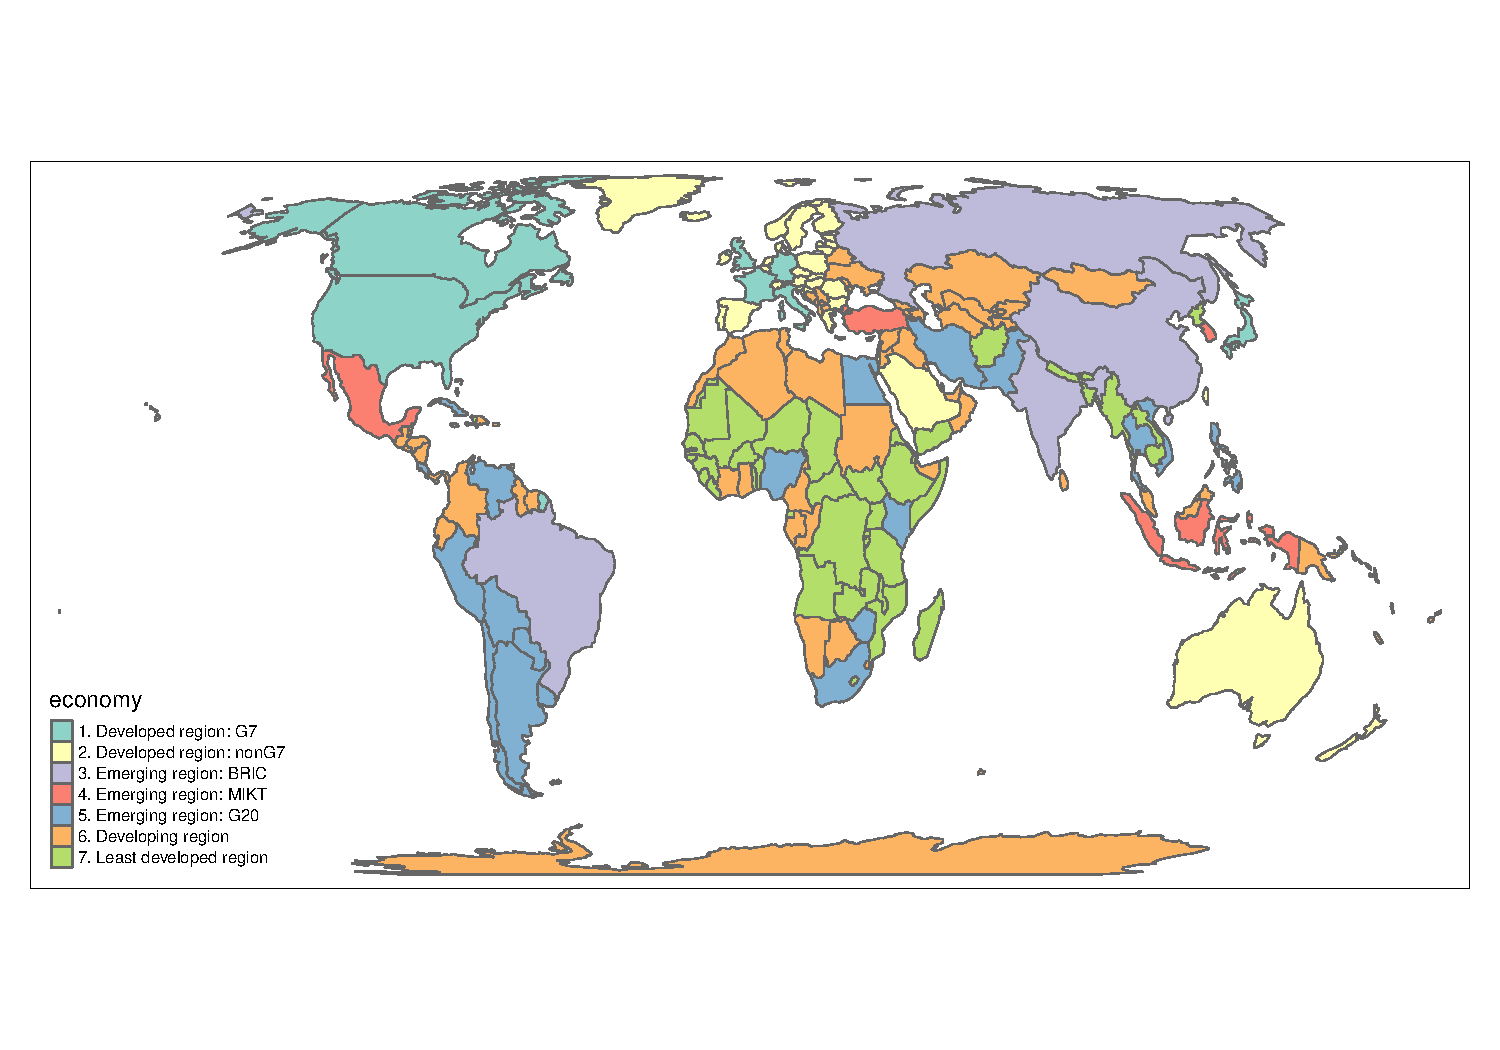
\includegraphics{quick_high_quality_maps_files/figure-beamer/unnamed-chunk-6-1.pdf}
\end{block}
\end{frame}

\begin{frame}{Topics of the World dataset}
\protect\hypertarget{topics-of-the-world-dataset}{}
\begin{block}{Available variables in the data set}
\protect\hypertarget{available-variables-in-the-data-set}{}
\begin{itemize}
\tightlist
\item
  \href{http://userpage.chemie.fu-berlin.de/diverse/doc/ISO_3166.html}{\textbf{ISO
  classification}}
\item
  country name
\item
  Area, population, population density,
\item
  \href{https://en.wikipedia.org/wiki/Gross_domestic_product}{\textbf{Gross
  Domestic Product}}
\item
  Gross domestic product
  \href{https://en.wikipedia.org/wiki/List_of_countries_by_GDP_\%28PPP\%29_per_capita}{\textbf{at
  purchasing power parities}}
\item
  Economy, income group
\end{itemize}
\end{block}

\begin{block}{\href{http://rpubs.com/Japhilko82/tmap_europe_dataset}{\textbf{Variables
of the World Dataset}}}
\protect\hypertarget{variables-of-the-world-dataset}{}
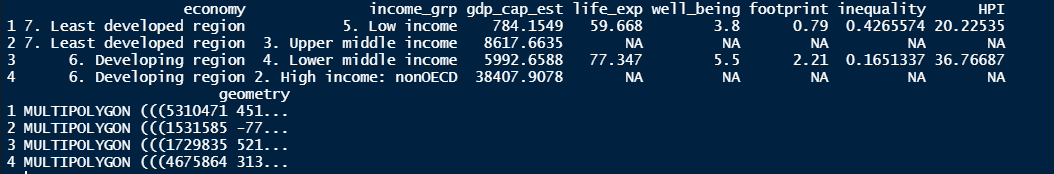
\includegraphics{pics/world_dataset.PNG}
\end{block}
\end{frame}

\begin{frame}[fragile]{The variable \texttt{continent}}
\protect\hypertarget{the-variable-continent}{}
\begin{Shaded}
\begin{Highlighting}[]
\KeywordTok{qtm}\NormalTok{(World, }\DataTypeTok{fill=}\StringTok{"continent"}\NormalTok{)}
\end{Highlighting}
\end{Shaded}

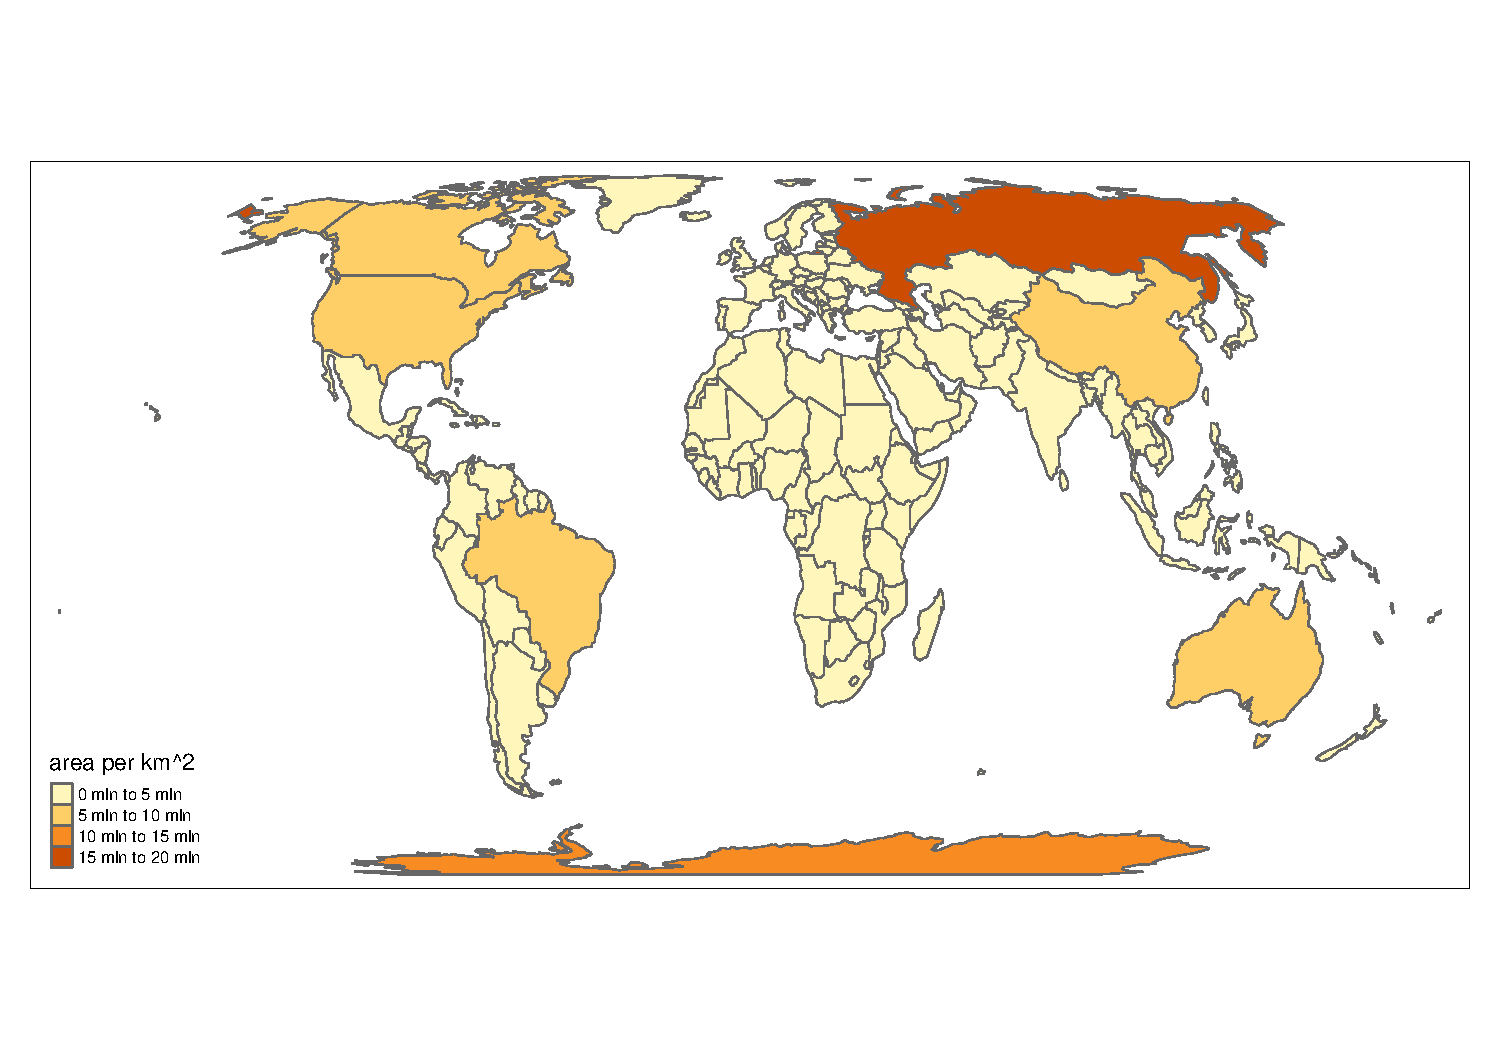
\includegraphics{quick_high_quality_maps_files/figure-beamer/unnamed-chunk-7-1.pdf}
\end{frame}

\begin{frame}[fragile]{The variable \texttt{area}}
\protect\hypertarget{the-variable-area}{}
\begin{Shaded}
\begin{Highlighting}[]
\KeywordTok{qtm}\NormalTok{(World, }\DataTypeTok{fill=}\StringTok{"area"}\NormalTok{) }\CommentTok{\# Russia is huge}
\end{Highlighting}
\end{Shaded}

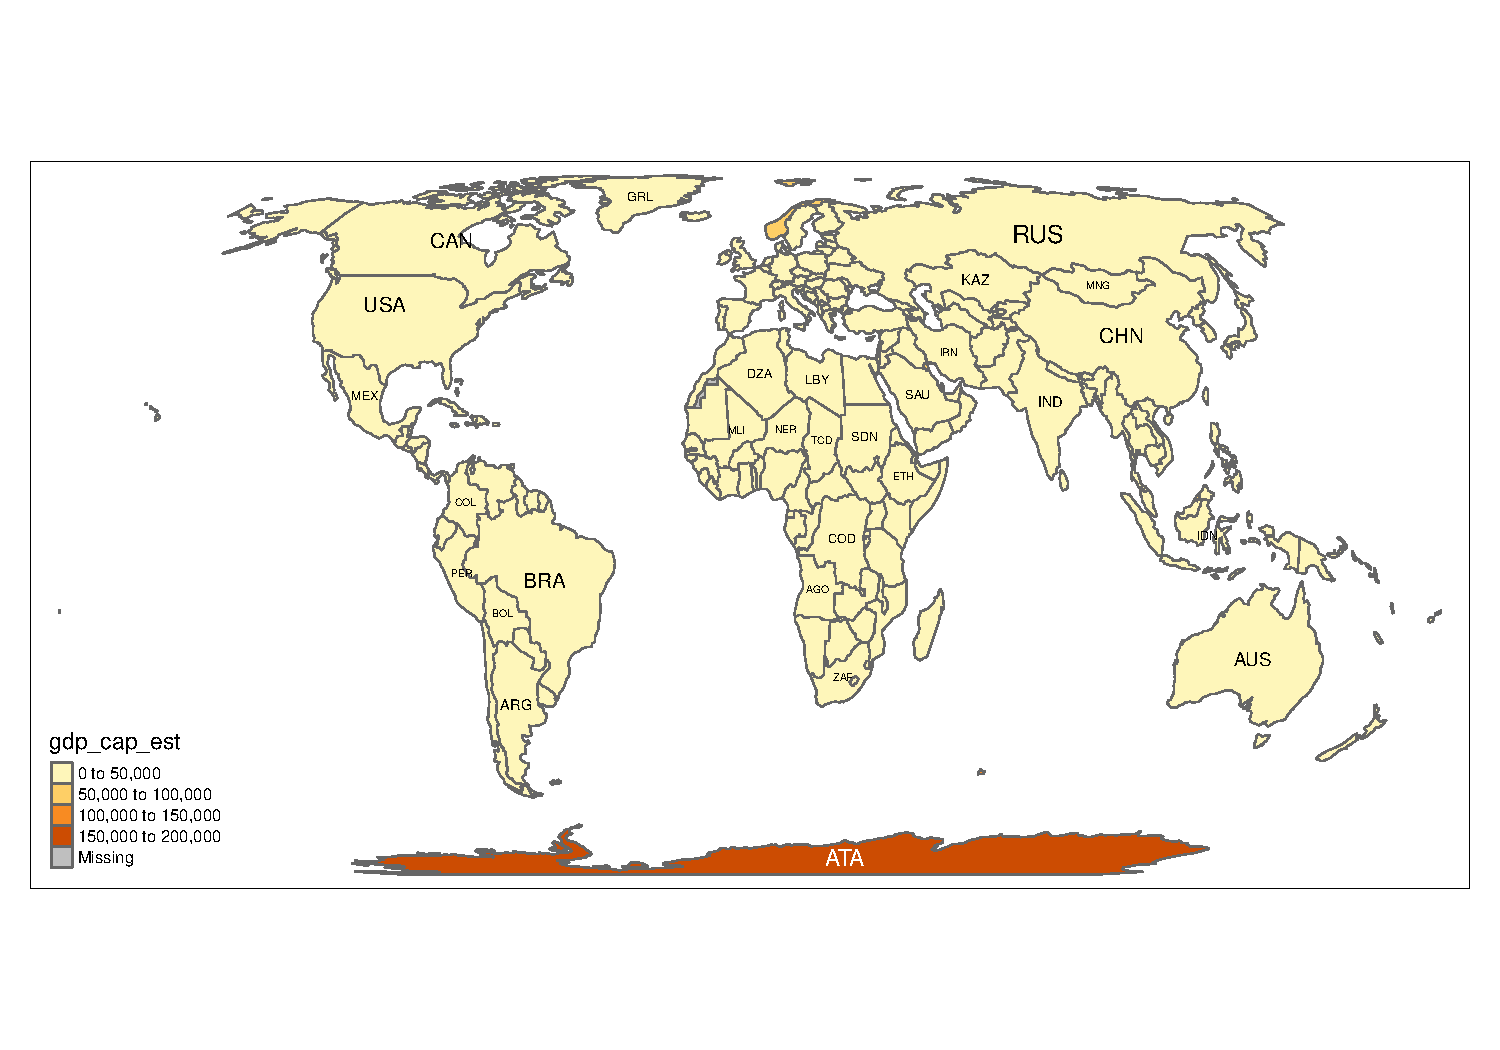
\includegraphics{quick_high_quality_maps_files/figure-beamer/unnamed-chunk-9-1.pdf}
\end{frame}

\begin{frame}[fragile]{Population}
\protect\hypertarget{population-1}{}
\begin{Shaded}
\begin{Highlighting}[]
\KeywordTok{qtm}\NormalTok{(World, }\DataTypeTok{fill=}\StringTok{"pop\_est"}\NormalTok{,}\DataTypeTok{fill.title=}\StringTok{"Population"}\NormalTok{) }
\end{Highlighting}
\end{Shaded}

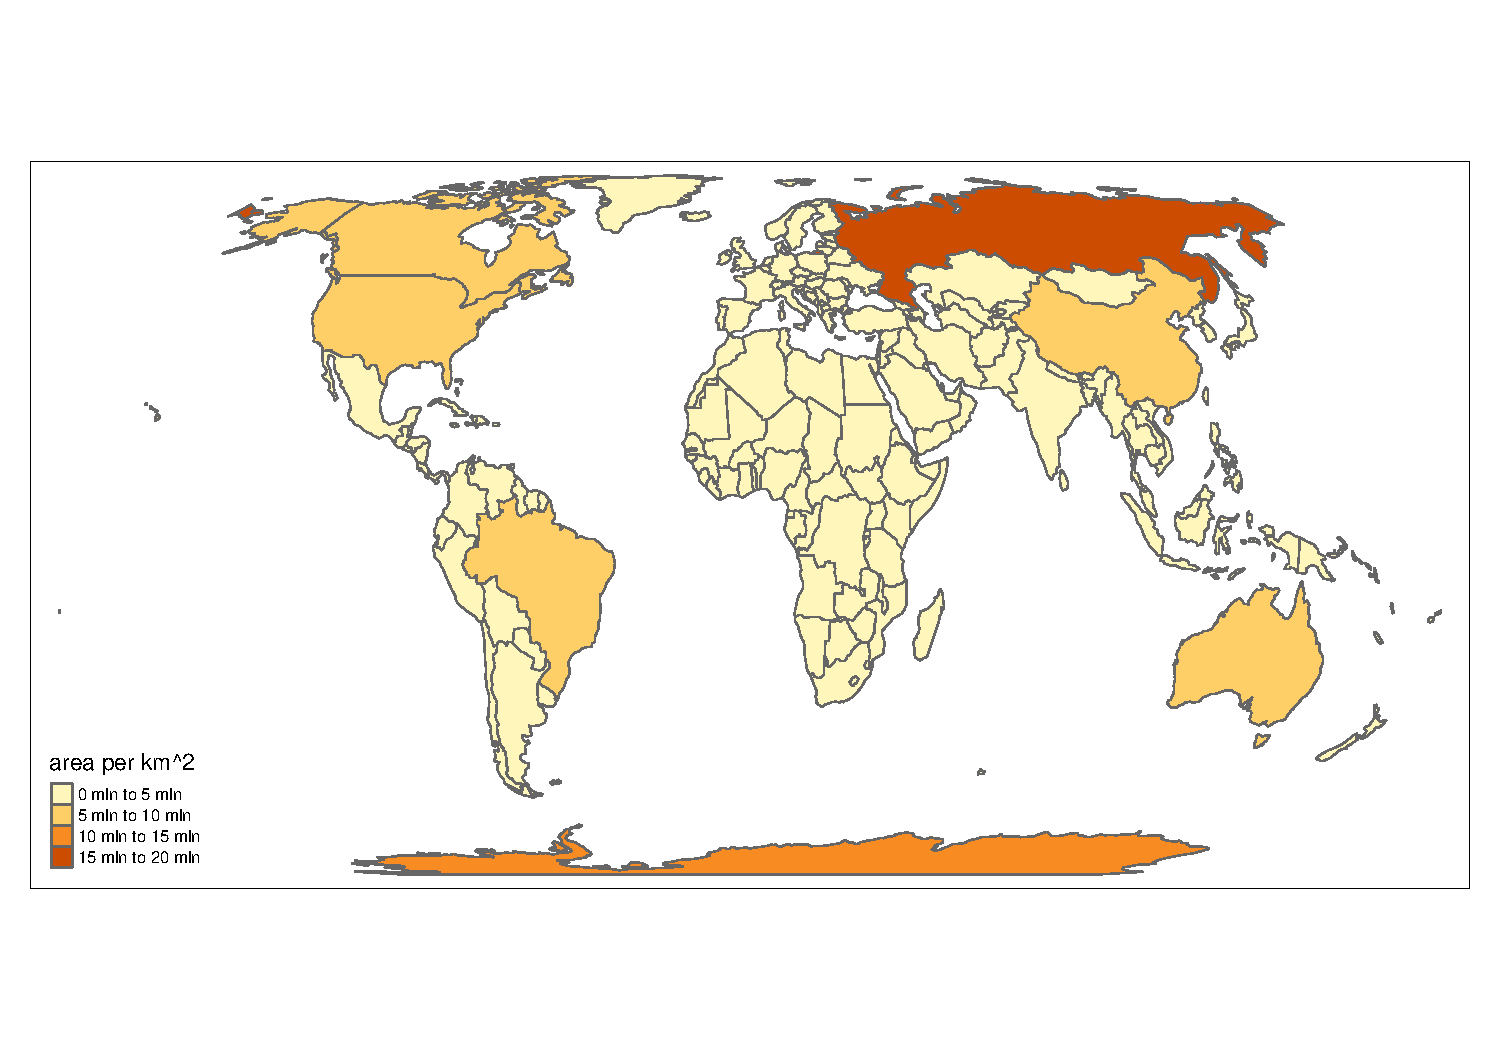
\includegraphics{quick_high_quality_maps_files/figure-beamer/unnamed-chunk-10-1.pdf}
\end{frame}

\begin{frame}[fragile]{Two maps}
\protect\hypertarget{two-maps}{}
\begin{block}{Population and level of development}
\protect\hypertarget{population-and-level-of-development}{}
\begin{Shaded}
\begin{Highlighting}[]
\KeywordTok{tm\_shape}\NormalTok{(World) }\OperatorTok{+}\StringTok{ }\KeywordTok{tm\_fill}\NormalTok{(}\KeywordTok{c}\NormalTok{(}\StringTok{"pop\_est"}\NormalTok{, }\StringTok{"economy"}\NormalTok{), }
        \DataTypeTok{title=}\KeywordTok{c}\NormalTok{(}\StringTok{"Population"}\NormalTok{, }\StringTok{"Economy"}\NormalTok{))}
\end{Highlighting}
\end{Shaded}

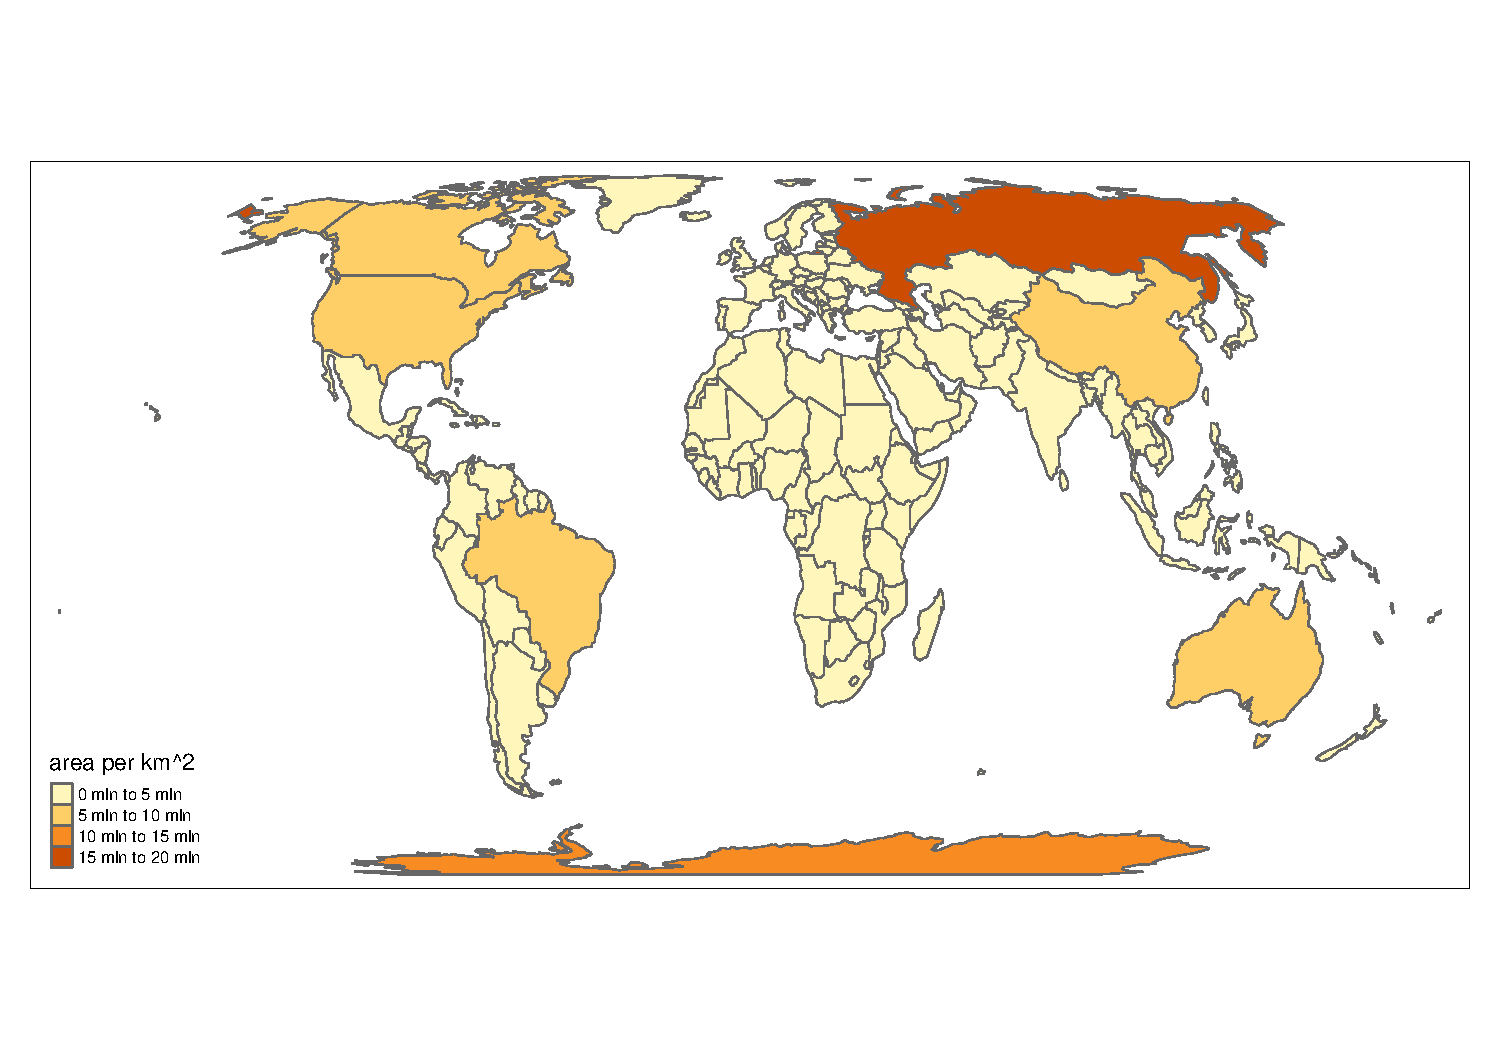
\includegraphics{quick_high_quality_maps_files/figure-beamer/unnamed-chunk-11-1.pdf}
\end{block}
\end{frame}

\begin{frame}[fragile]{Netherlands - Population in the provinces}
\protect\hypertarget{netherlands---population-in-the-provinces}{}
\begin{Shaded}
\begin{Highlighting}[]
\KeywordTok{data}\NormalTok{(land)}
\KeywordTok{data}\NormalTok{(World)}
\end{Highlighting}
\end{Shaded}

\begin{Shaded}
\begin{Highlighting}[]
\KeywordTok{tm\_shape}\NormalTok{(land,  }\DataTypeTok{relative=}\OtherTok{FALSE}\NormalTok{) }\OperatorTok{+}
\StringTok{    }\KeywordTok{tm\_raster}\NormalTok{(}\StringTok{"trees"}\NormalTok{, }\DataTypeTok{title=}\StringTok{"prop. wooded area"}\NormalTok{)}
\end{Highlighting}
\end{Shaded}

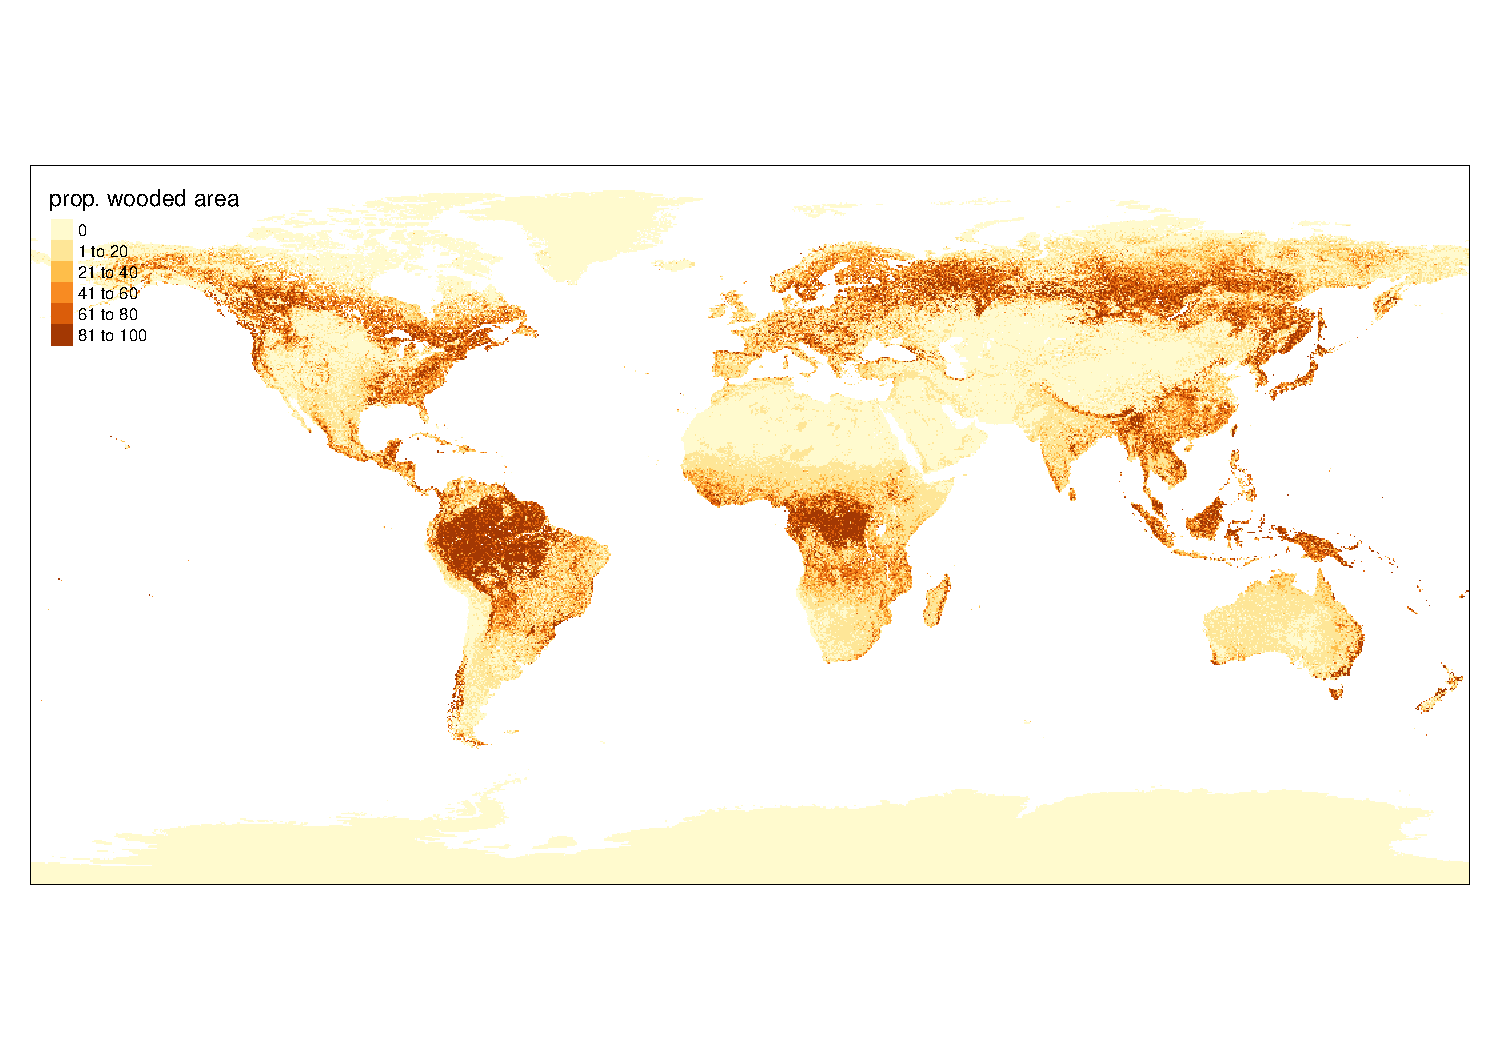
\includegraphics{quick_high_quality_maps_files/figure-beamer/unnamed-chunk-15-1.pdf}
\end{frame}

\begin{frame}[fragile]{Visualize only one country}
\protect\hypertarget{visualize-only-one-country}{}
\begin{Shaded}
\begin{Highlighting}[]
\KeywordTok{tm\_shape}\NormalTok{(World[World}\OperatorTok{$}\NormalTok{name}\OperatorTok{==}\StringTok{"Austria"}\NormalTok{, ]) }\OperatorTok{+}
\StringTok{    }\KeywordTok{tm\_polygons}\NormalTok{()}
\end{Highlighting}
\end{Shaded}

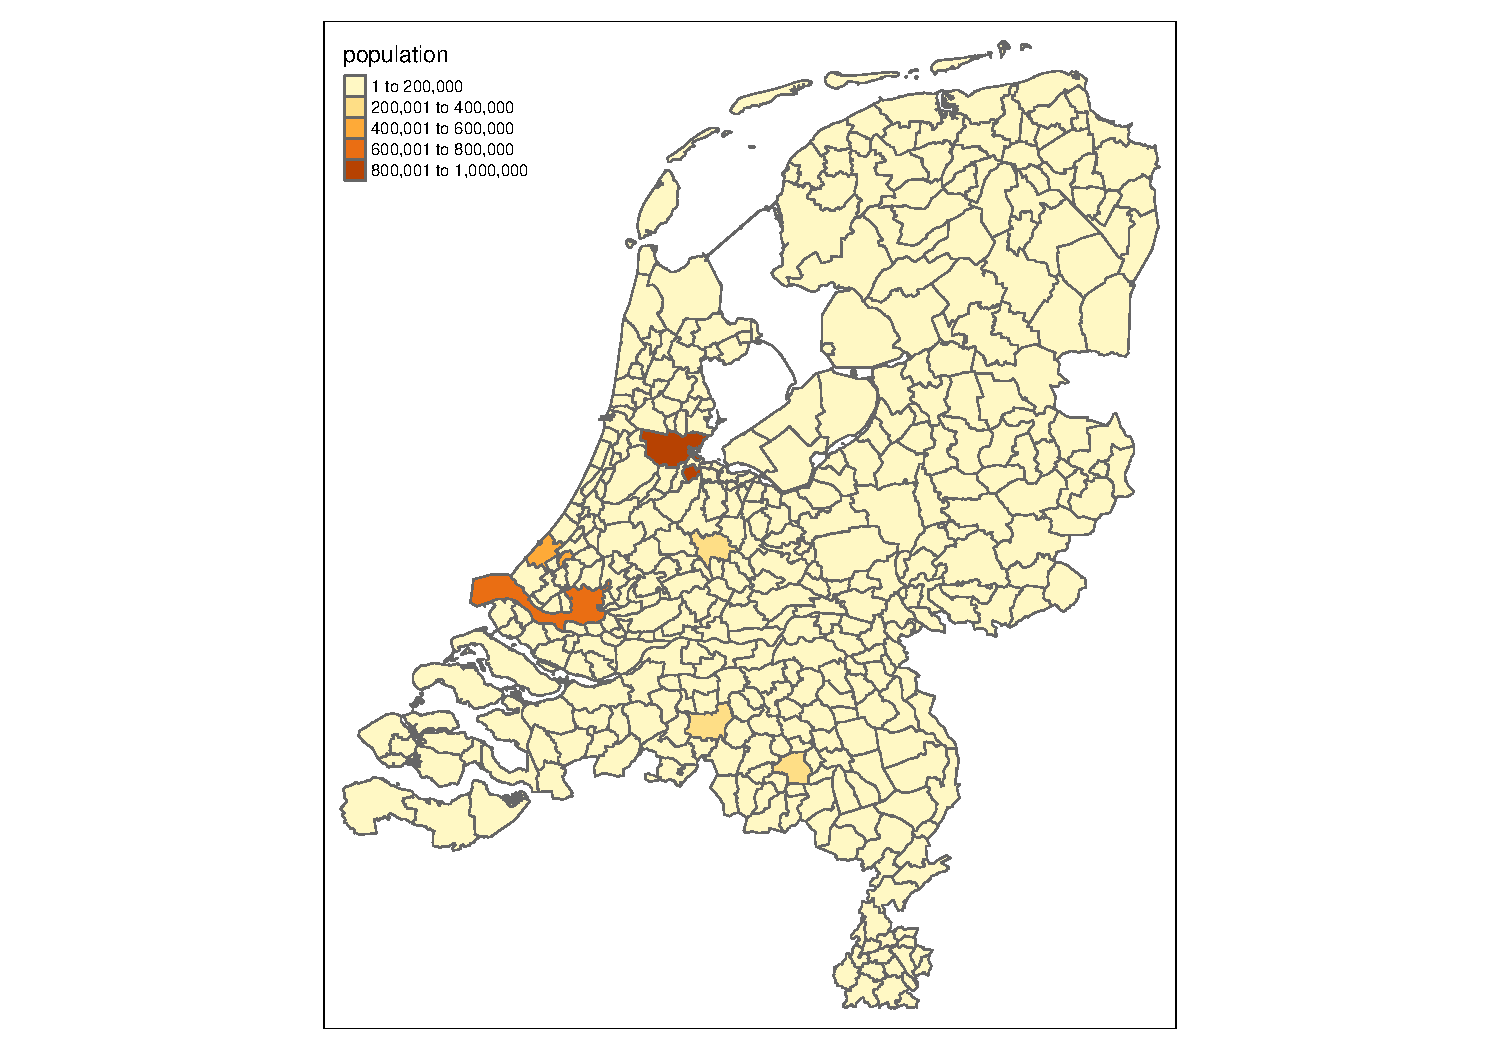
\includegraphics{quick_high_quality_maps_files/figure-beamer/unnamed-chunk-16-1.pdf}
\end{frame}

\begin{frame}{The \texttt{raster} package}
\protect\hypertarget{the-raster-package}{}
Title: Geographic Data Analysis and Modeling

Description: Reading, writing, manipulating, analyzing and modeling of
spatial data. The package implements basic and high-level functions for
raster data and for vector data operations such as intersections.

Author: Robert J. Hijmans {[}cre, aut{]}
(\url{https://orcid.org/0000-0001-5872-2872}), Jacob van Etten
{[}ctb{]}, Michael Sumner {[}ctb{]}, Joe Cheng {[}ctb{]}, Dan Baston
{[}ctb{]}, Andrew Bevan {[}ctb{]}, Roger Bivand {[}ctb{]}, Lorenzo
Busetto {[}ctb{]}, Mort Canty {[}ctb{]}, David Forrest {[}ctb{]},
Aniruddha Ghosh {[}ctb{]}, Duncan Golicher {[}ctb{]}, Josh Gray
{[}ctb{]}, Jonathan A. Greenberg {[}ctb{]}, Paul Hiemstra {[}ctb{]},
Kassel Hingee {[}ctb{]}, Institute for Mathematics Applied Geosciences
{[}cph{]}, Charles Karney {[}ctb{]}, Matteo Mattiuzzi {[}ctb{]}, Steven
Mosher {[}ctb{]},
\end{frame}

\begin{frame}[fragile]{Global Administrative Boundaries}
\protect\hypertarget{global-administrative-boundaries}{}
\begin{block}{Get the data}
\protect\hypertarget{get-the-data}{}
\begin{Shaded}
\begin{Highlighting}[]
\NormalTok{FRA4 \textless{}{-}}\StringTok{ }\NormalTok{raster}\OperatorTok{::}\KeywordTok{getData}\NormalTok{(}\StringTok{\textquotesingle{}GADM\textquotesingle{}}\NormalTok{, }\DataTypeTok{country=}\StringTok{\textquotesingle{}FRA\textquotesingle{}}\NormalTok{, }
                        \DataTypeTok{level=}\DecValTok{4}\NormalTok{)}
\end{Highlighting}
\end{Shaded}
\end{block}

\begin{block}{\href{https://rpubs.com/Jan-Philipp_Kolb/FRA4}{\textbf{Overview
of the data}}}
\protect\hypertarget{overview-of-the-data}{}
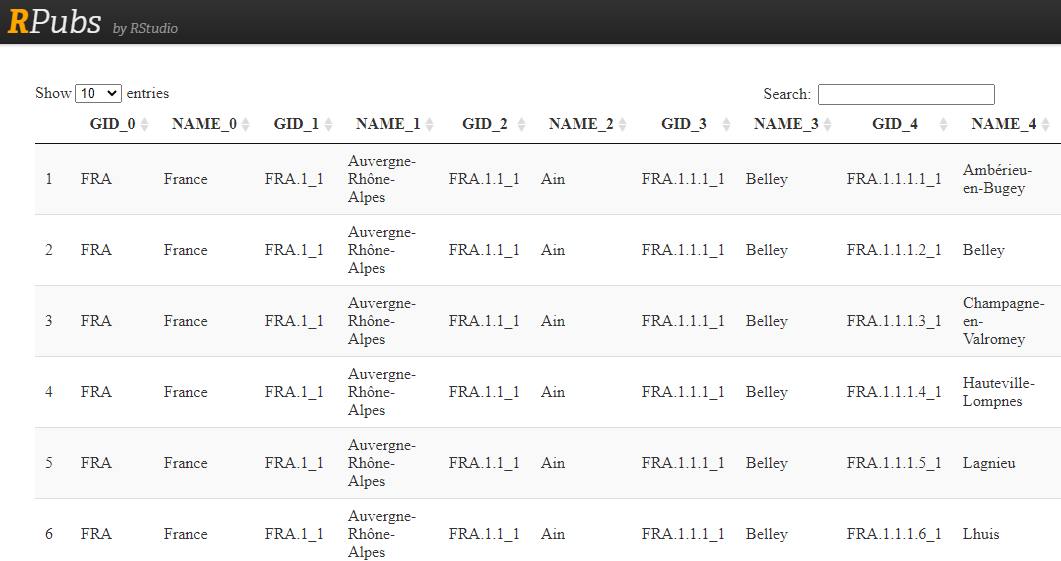
\includegraphics{pics/FRA4_data_rpubs.PNG}
\end{block}
\end{frame}

\begin{frame}[fragile]{Plot the map}
\protect\hypertarget{plot-the-map}{}
\begin{Shaded}
\begin{Highlighting}[]
\KeywordTok{qtm}\NormalTok{(FRA4,}\DataTypeTok{fill=}\StringTok{"blue"}\NormalTok{)}
\end{Highlighting}
\end{Shaded}

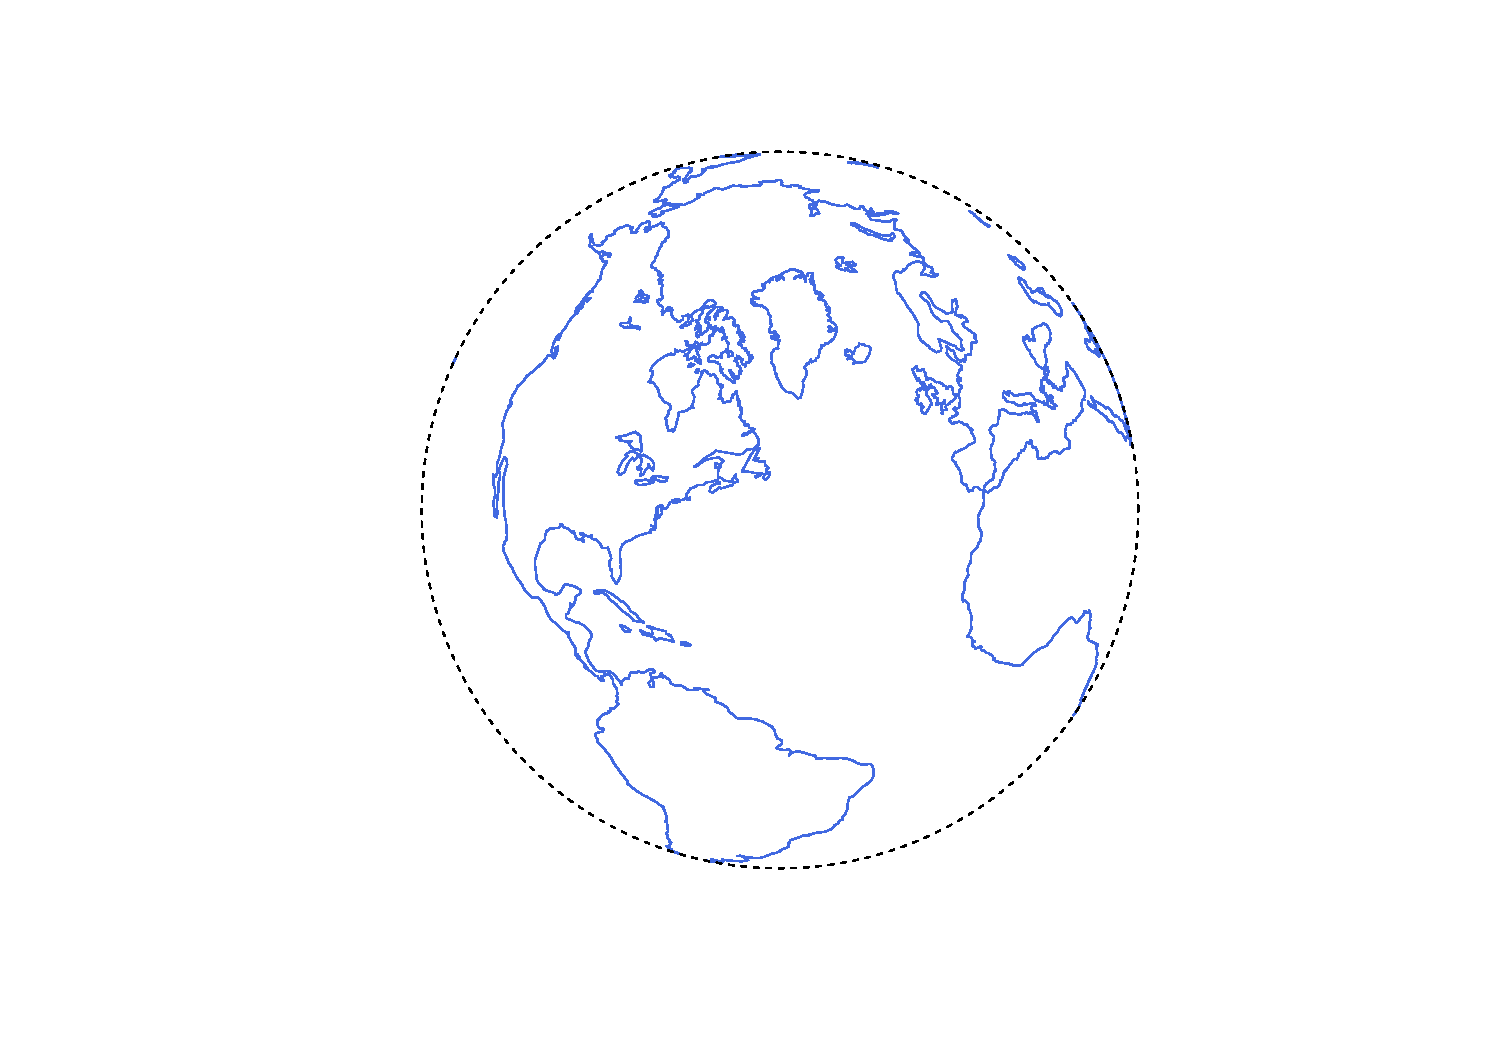
\includegraphics{quick_high_quality_maps_files/figure-beamer/unnamed-chunk-20-1.pdf}
\end{frame}

\begin{frame}[fragile]{Create colour gradiation}
\protect\hypertarget{create-colour-gradiation}{}
\begin{Shaded}
\begin{Highlighting}[]
\NormalTok{FRA4}\OperatorTok{$}\NormalTok{fantasy\_val \textless{}{-}}\StringTok{ }\KeywordTok{runif}\NormalTok{(}\KeywordTok{nrow}\NormalTok{(FRA4))}
  \KeywordTok{qtm}\NormalTok{(FRA4,}\StringTok{"fantasy\_val"}\NormalTok{, }
      \DataTypeTok{fill.palette =} \KeywordTok{rgb}\NormalTok{(}\DecValTok{0}\NormalTok{,}\DecValTok{0}\NormalTok{,}\KeywordTok{seq}\NormalTok{(}\DecValTok{0}\NormalTok{,}\DecValTok{1}\NormalTok{,.}\DecValTok{1}\NormalTok{),}\DecValTok{0}\NormalTok{),}
      \DataTypeTok{borders =} \StringTok{"blue"}\NormalTok{)}
\end{Highlighting}
\end{Shaded}

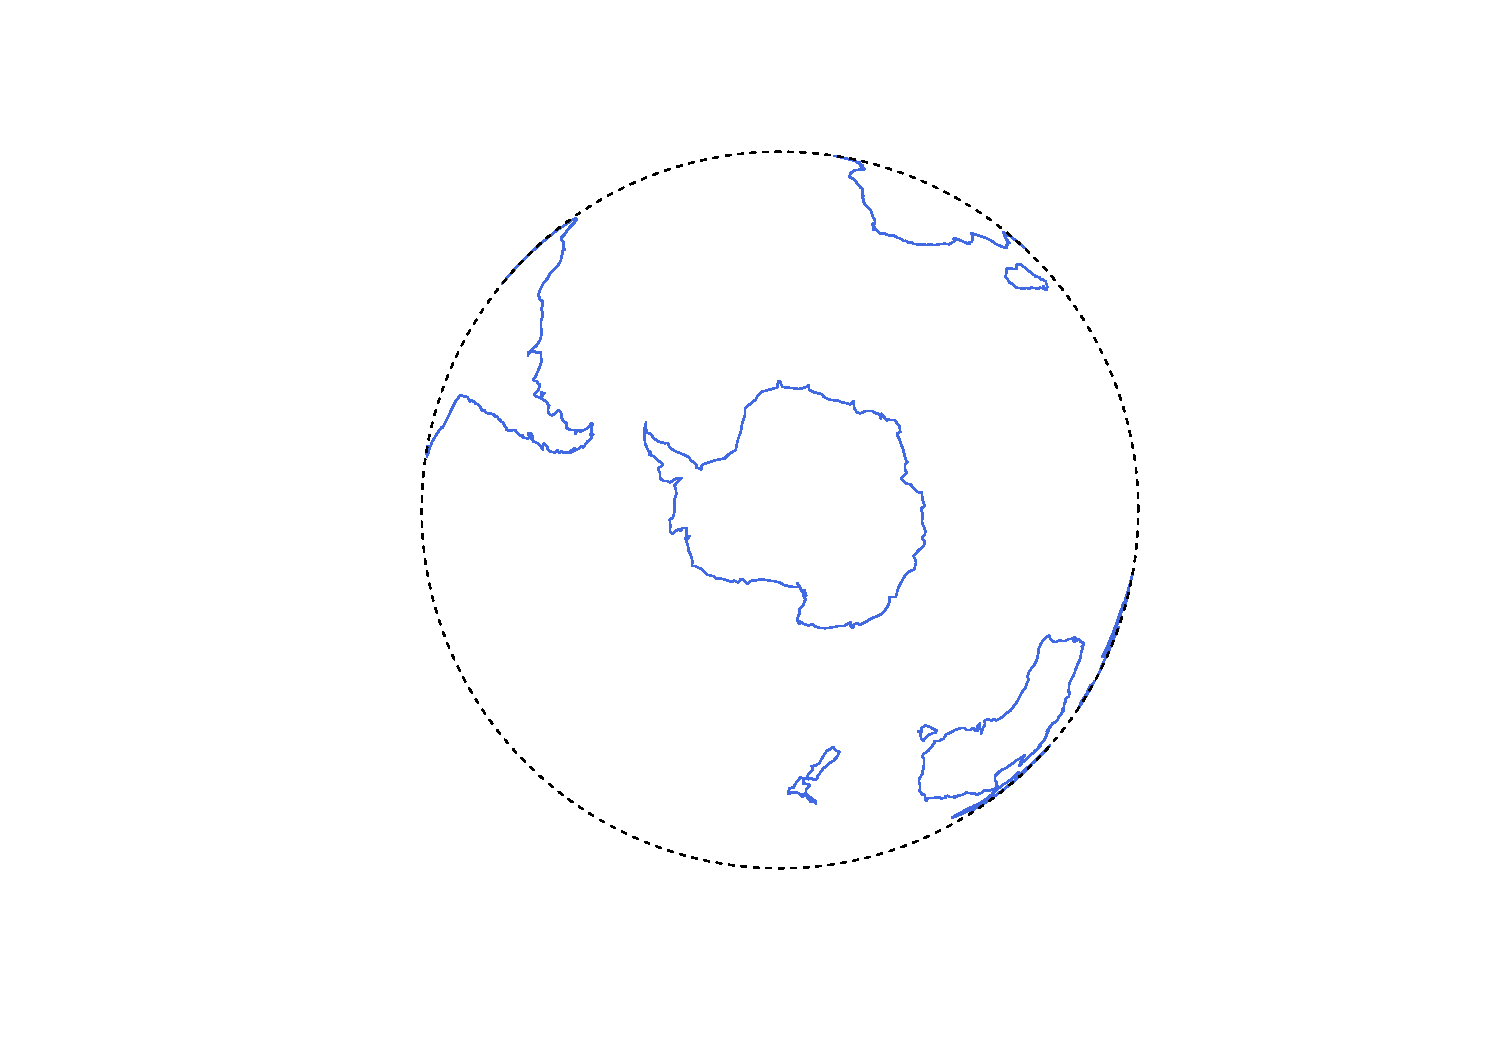
\includegraphics{quick_high_quality_maps_files/figure-beamer/unnamed-chunk-21-1.pdf}
\end{frame}

\begin{frame}{Longitude and Latitude}
\protect\hypertarget{longitude-and-latitude}{}
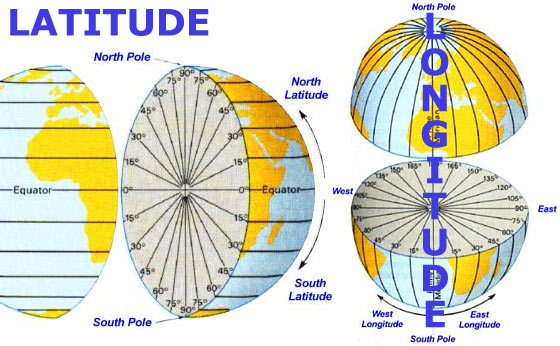
\includegraphics{pics/definition-of-latitude-longitude.PNG}
\end{frame}

\begin{frame}[fragile]{\texttt{tmaptools} - Thematic Map Tools}
\protect\hypertarget{tmaptools---thematic-map-tools}{}
\begin{Shaded}
\begin{Highlighting}[]
\KeywordTok{library}\NormalTok{(tmaptools)}
\end{Highlighting}
\end{Shaded}

Author: Martijn Tennekes

\begin{Shaded}
\begin{Highlighting}[]
\KeywordTok{citation}\NormalTok{(}\StringTok{"tmaptools"}\NormalTok{)}
\end{Highlighting}
\end{Shaded}

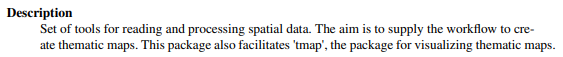
\includegraphics{pics/description_tmaptools.PNG}
\end{frame}

\begin{frame}[fragile]{Geocoordinates}
\protect\hypertarget{geocoordinates}{}
\begin{Shaded}
\begin{Highlighting}[]
\NormalTok{(gc\_z \textless{}{-}}\StringTok{ }\KeywordTok{geocode\_OSM}\NormalTok{(}\StringTok{"Zürich"}\NormalTok{))}
\end{Highlighting}
\end{Shaded}

\begin{verbatim}
## $query
## [1] "Zürich"
## 
## $coords
##         x         y 
##  8.541042 47.374449 
## 
## $bbox
##      xmin      ymin      xmax      ymax 
##  8.448006 47.320220  8.625441 47.434666
\end{verbatim}
\end{frame}

\begin{frame}[fragile]{A package to get Openstreetmap data}
\protect\hypertarget{a-package-to-get-openstreetmap-data}{}
Author: Mark Padgham

\begin{Shaded}
\begin{Highlighting}[]
\KeywordTok{library}\NormalTok{(osmplotr)}
\end{Highlighting}
\end{Shaded}

\begin{Shaded}
\begin{Highlighting}[]
\KeywordTok{citation}\NormalTok{(}\StringTok{"osmplotr"}\NormalTok{)}
\end{Highlighting}
\end{Shaded}

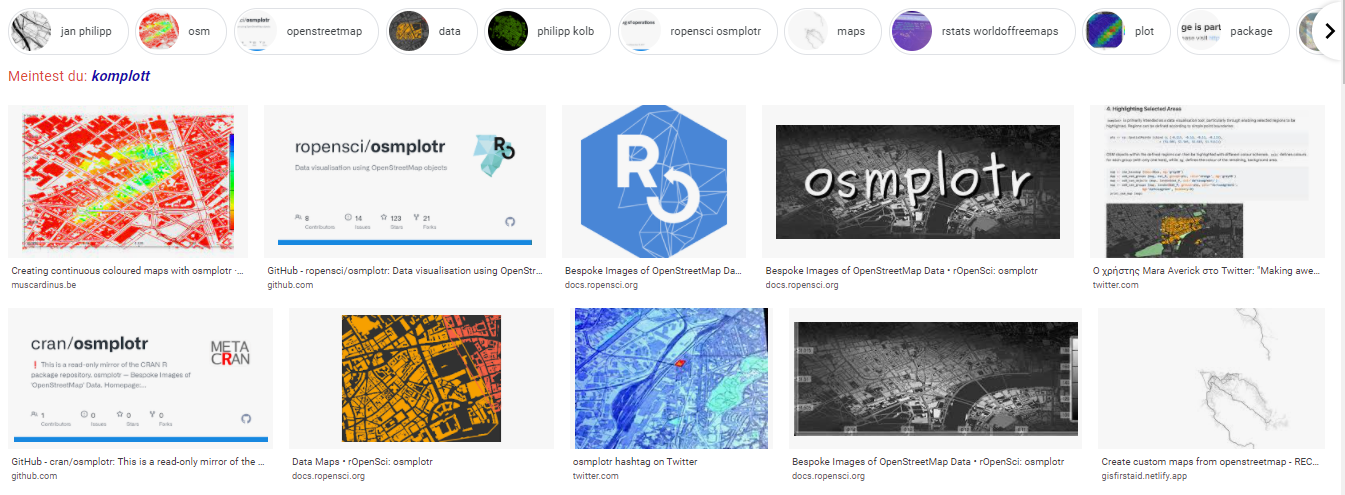
\includegraphics{pics/osmplotr_google.png}
\end{frame}

\begin{frame}[fragile]{Buildings within a bounding box}
\protect\hypertarget{buildings-within-a-bounding-box}{}
\begin{Shaded}
\begin{Highlighting}[]
\NormalTok{bbox \textless{}{-}}\StringTok{ }\KeywordTok{get\_bbox}\NormalTok{ (}\KeywordTok{c}\NormalTok{(}\FloatTok{8.4539}\NormalTok{ , }\FloatTok{49.4805}\NormalTok{  , }
                    \FloatTok{8.4774}\NormalTok{ , }\FloatTok{49.4943}\NormalTok{ ))}
\NormalTok{dat\_M \textless{}{-}}\StringTok{ }\KeywordTok{extract\_osm\_objects}\NormalTok{ (}\DataTypeTok{key =} \StringTok{\textquotesingle{}building\textquotesingle{}}\NormalTok{, }
                              \DataTypeTok{bbox =}\NormalTok{ bbox)}
\end{Highlighting}
\end{Shaded}

\begin{Shaded}
\begin{Highlighting}[]
\KeywordTok{qtm}\NormalTok{(dat\_M,}\DataTypeTok{fill=}\KeywordTok{c}\NormalTok{(}\StringTok{"purple"}\NormalTok{),}\DataTypeTok{borders=}\StringTok{"black"}\NormalTok{)}
\end{Highlighting}
\end{Shaded}

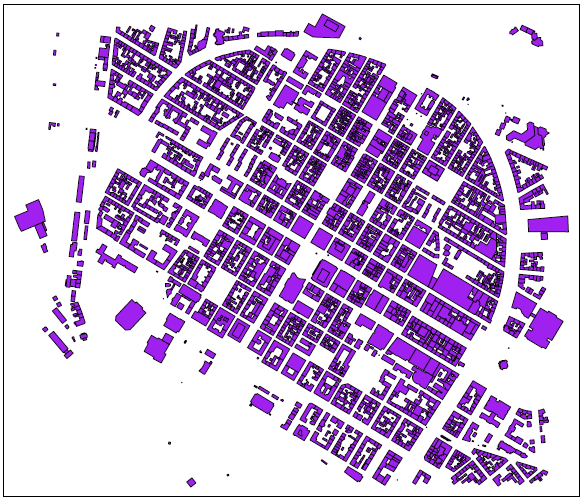
\includegraphics[width=0.5\textwidth,height=\textheight]{pics/bui_mannheim.PNG}
\end{frame}

\begin{frame}{Colour picker}
\protect\hypertarget{colour-picker}{}
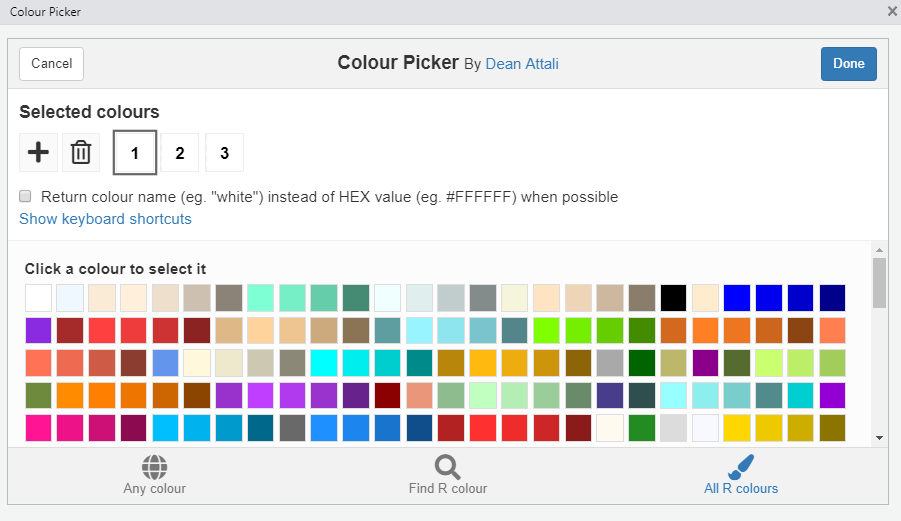
\includegraphics{pics/colourpicker.png}
\end{frame}

\begin{frame}[fragile]{The package \texttt{osmdata}}
\protect\hypertarget{the-package-osmdata}{}
\begin{Shaded}
\begin{Highlighting}[]
\KeywordTok{install.packages}\NormalTok{(}\StringTok{"osmdata"}\NormalTok{)}
\end{Highlighting}
\end{Shaded}

\begin{Shaded}
\begin{Highlighting}[]
\KeywordTok{library}\NormalTok{(osmdata)}
\end{Highlighting}
\end{Shaded}

\begin{block}{Get a bounding box for a city}
\protect\hypertarget{get-a-bounding-box-for-a-city}{}
\begin{Shaded}
\begin{Highlighting}[]
\NormalTok{bbox \textless{}{-}}\StringTok{ }\KeywordTok{getbb}\NormalTok{(}\StringTok{"Berlin"}\NormalTok{)}
\end{Highlighting}
\end{Shaded}
\end{block}
\end{frame}

\begin{frame}[fragile]{Streets of Berlin}
\protect\hypertarget{streets-of-berlin}{}
\begin{block}{OSM Map Feature key=highway value=primary}
\protect\hypertarget{osm-map-feature-keyhighway-valueprimary}{}
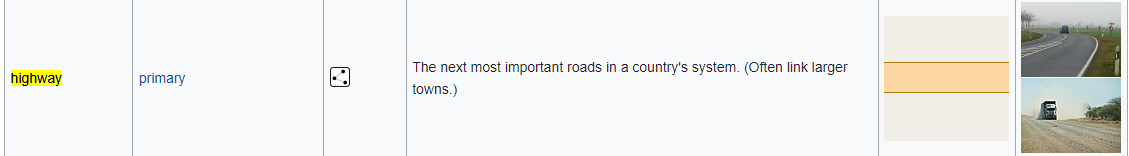
\includegraphics{pics/highway_primary_osmmapfeatures.PNG}
\end{block}

\begin{block}{Get data with package \texttt{osmdata}}
\protect\hypertarget{get-data-with-package-osmdata}{}
\begin{Shaded}
\begin{Highlighting}[]
\NormalTok{dat \textless{}{-}}\StringTok{ }\KeywordTok{extract\_osm\_objects}\NormalTok{(}\DataTypeTok{key =} \StringTok{\textquotesingle{}highway\textquotesingle{}}\NormalTok{,}
                              \DataTypeTok{value =} \StringTok{"primary"}\NormalTok{,}
                              \DataTypeTok{bbox =}\NormalTok{ bbox)}
\end{Highlighting}
\end{Shaded}
\end{block}
\end{frame}

\begin{frame}[fragile]{A quick map for the primary streets in Berlin}
\protect\hypertarget{a-quick-map-for-the-primary-streets-in-berlin}{}
\begin{Shaded}
\begin{Highlighting}[]
\KeywordTok{qtm}\NormalTok{(dat)}
\end{Highlighting}
\end{Shaded}

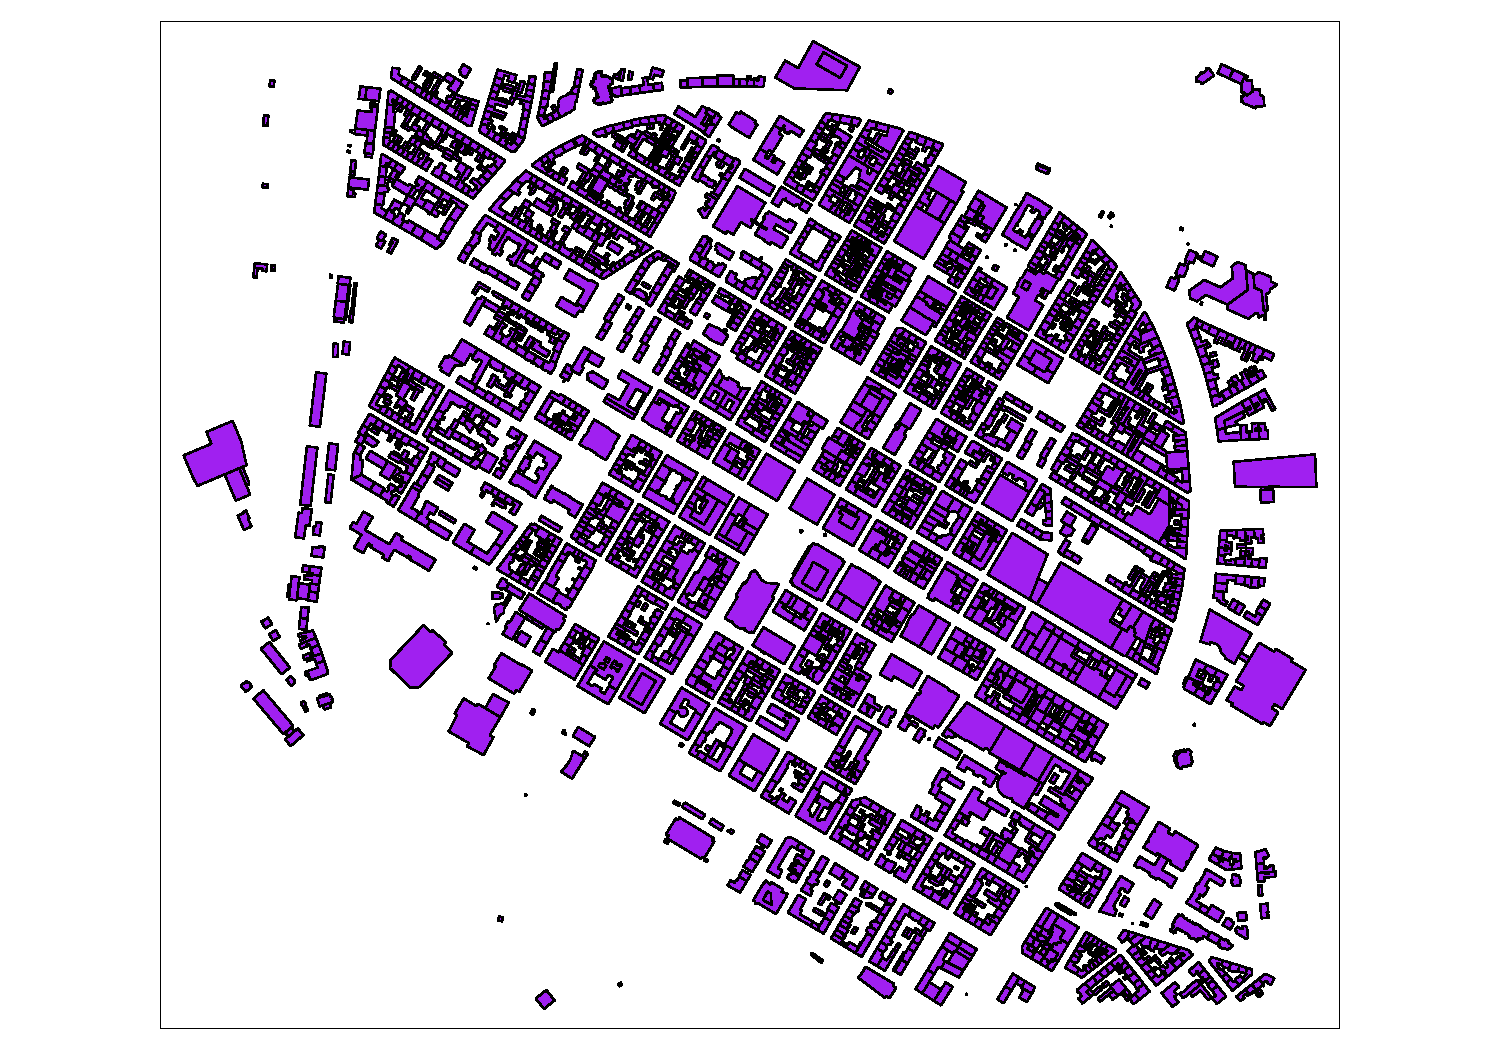
\includegraphics{quick_high_quality_maps_files/figure-beamer/unnamed-chunk-37-1.pdf}
\end{frame}

\begin{frame}[fragile]{}
\protect\hypertarget{section}{}
\begin{Shaded}
\begin{Highlighting}[]
\NormalTok{dat\_s \textless{}{-}}\StringTok{ }\KeywordTok{extract\_osm\_objects}\NormalTok{(}\DataTypeTok{key =} \StringTok{\textquotesingle{}highway\textquotesingle{}}\NormalTok{,}
                           \DataTypeTok{value =} \StringTok{"secondary"}\NormalTok{,}
                           \DataTypeTok{bbox =}\NormalTok{ bbox)}
\end{Highlighting}
\end{Shaded}

\begin{Shaded}
\begin{Highlighting}[]
\NormalTok{map \textless{}{-}}\StringTok{ }\KeywordTok{osm\_basemap}\NormalTok{(}\DataTypeTok{bbox =}\NormalTok{ bbox, }\DataTypeTok{bg =} \StringTok{"\#F5F5DC"}\NormalTok{)}
\NormalTok{map \textless{}{-}}\StringTok{ }\KeywordTok{add\_osm\_objects}\NormalTok{(map, dat, }\DataTypeTok{col =} \StringTok{"\#00008B"}\NormalTok{)}
\NormalTok{map \textless{}{-}}\StringTok{ }\KeywordTok{add\_osm\_objects}\NormalTok{(map, dat\_s, }\DataTypeTok{col =} \StringTok{"purple"}\NormalTok{)}
\KeywordTok{print\_osm\_map}\NormalTok{(map)}
\end{Highlighting}
\end{Shaded}
\end{frame}

\begin{frame}{30daymapchallenge}
\protect\hypertarget{daymapchallenge}{}
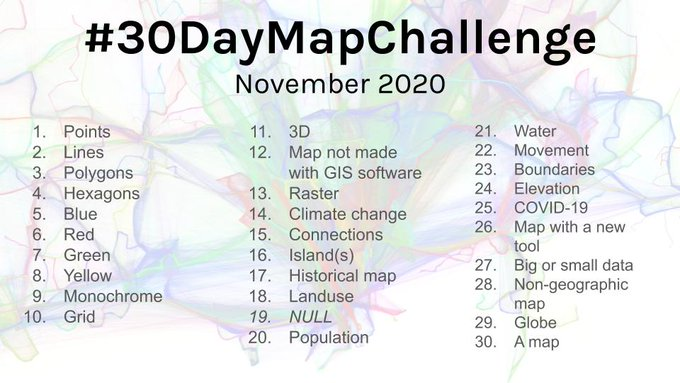
\includegraphics{pics/30daymapchallenge_copy_1jpg}
\end{frame}

\begin{frame}{Day 9 monochrome}
\protect\hypertarget{day-9-monochrome}{}
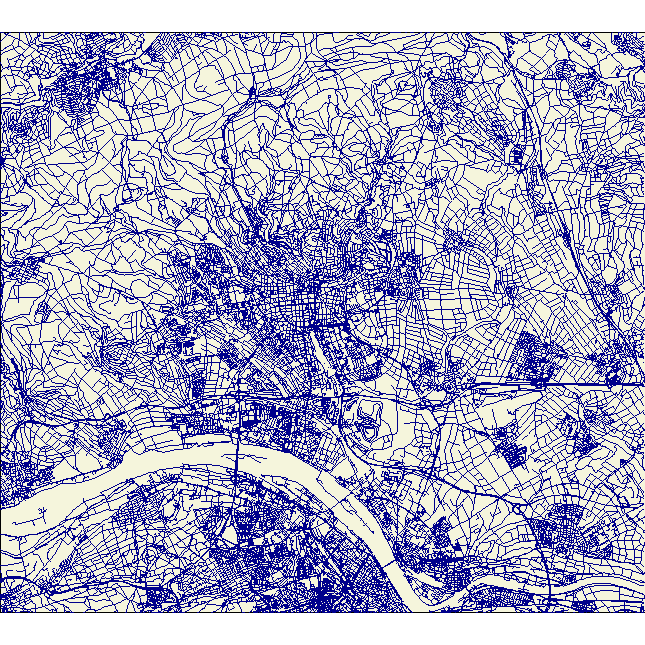
\includegraphics{pics/trier_monochrome.png}
\end{frame}

\begin{frame}[fragile]{Load example data}
\protect\hypertarget{load-example-data}{}
\begin{block}{Data source Eurostat}
\protect\hypertarget{data-source-eurostat}{}
\begin{itemize}
\tightlist
\item
  Data about unemployment in Europe
\end{itemize}

\begin{Shaded}
\begin{Highlighting}[]
\NormalTok{url \textless{}{-}}\StringTok{ "https://raw.githubusercontent.com/Japhilko/}
\StringTok{GeoData/master/2015/data/Unemployment07a13.csv"}

\NormalTok{Unemp \textless{}{-}}\StringTok{ }\KeywordTok{read.csv}\NormalTok{(url) }
\end{Highlighting}
\end{Shaded}
\end{block}
\end{frame}

\begin{frame}[fragile]{Excursus: the command \texttt{match}}
\protect\hypertarget{excursus-the-command-match}{}
\begin{block}{Create two example vectors}
\protect\hypertarget{create-two-example-vectors}{}
\begin{Shaded}
\begin{Highlighting}[]
\NormalTok{vec\_a \textless{}{-}}\StringTok{ }\KeywordTok{c}\NormalTok{(}\StringTok{"A"}\NormalTok{,}\DecValTok{2}\NormalTok{,}\DecValTok{6}\NormalTok{,}\DecValTok{1}\NormalTok{,}\StringTok{"C"}\NormalTok{)}
\NormalTok{vec\_b \textless{}{-}}\StringTok{ }\KeywordTok{c}\NormalTok{(}\DecValTok{1}\NormalTok{,}\StringTok{"C"}\NormalTok{,}\DecValTok{2}\NormalTok{)}
\end{Highlighting}
\end{Shaded}
\end{block}

\begin{block}{Bringing the two vectors together}
\protect\hypertarget{bringing-the-two-vectors-together}{}
\begin{itemize}
\tightlist
\item
  With the function \texttt{match} you can see which element of the
  first vector matches the second vector.
\end{itemize}

\begin{Shaded}
\begin{Highlighting}[]
\KeywordTok{match}\NormalTok{(vec\_a,vec\_b)}
\end{Highlighting}
\end{Shaded}

\begin{verbatim}
## [1] NA  3 NA  1  2
\end{verbatim}
\end{block}
\end{frame}

\begin{frame}[fragile]{Use the package \texttt{tmap} with your data}
\protect\hypertarget{use-the-package-tmap-with-your-data}{}
\begin{Shaded}
\begin{Highlighting}[]
\KeywordTok{library}\NormalTok{(}\StringTok{"tmap"}\NormalTok{)}
\end{Highlighting}
\end{Shaded}

\begin{block}{Match the data}
\protect\hypertarget{match-the-data}{}
\begin{Shaded}
\begin{Highlighting}[]
\NormalTok{iso\_a2\textless{}{-}}\StringTok{ }\KeywordTok{substr}\NormalTok{(World}\OperatorTok{$}\NormalTok{iso\_a3,}\DecValTok{1}\NormalTok{,}\DecValTok{2}\NormalTok{)}
\NormalTok{ind \textless{}{-}}\StringTok{ }\KeywordTok{match}\NormalTok{(iso\_a2,Unemp}\OperatorTok{$}\NormalTok{GEO)}
\NormalTok{World}\OperatorTok{$}\NormalTok{Val2007M12 \textless{}{-}}\StringTok{ }\NormalTok{Unemp}\OperatorTok{$}\NormalTok{Val2007M12[ind]}
\NormalTok{World}\OperatorTok{$}\NormalTok{Val2013M01 \textless{}{-}}\StringTok{ }\NormalTok{Unemp}\OperatorTok{$}\NormalTok{Val2013M01[ind]}
\end{Highlighting}
\end{Shaded}
\end{block}
\end{frame}

\begin{frame}[fragile]{Plot a map}
\protect\hypertarget{plot-a-map}{}
\begin{Shaded}
\begin{Highlighting}[]
\KeywordTok{qtm}\NormalTok{(World,}\KeywordTok{c}\NormalTok{(}\StringTok{"Val2007M12"}\NormalTok{,}\StringTok{"Val2013M01"}\NormalTok{))}
\end{Highlighting}
\end{Shaded}

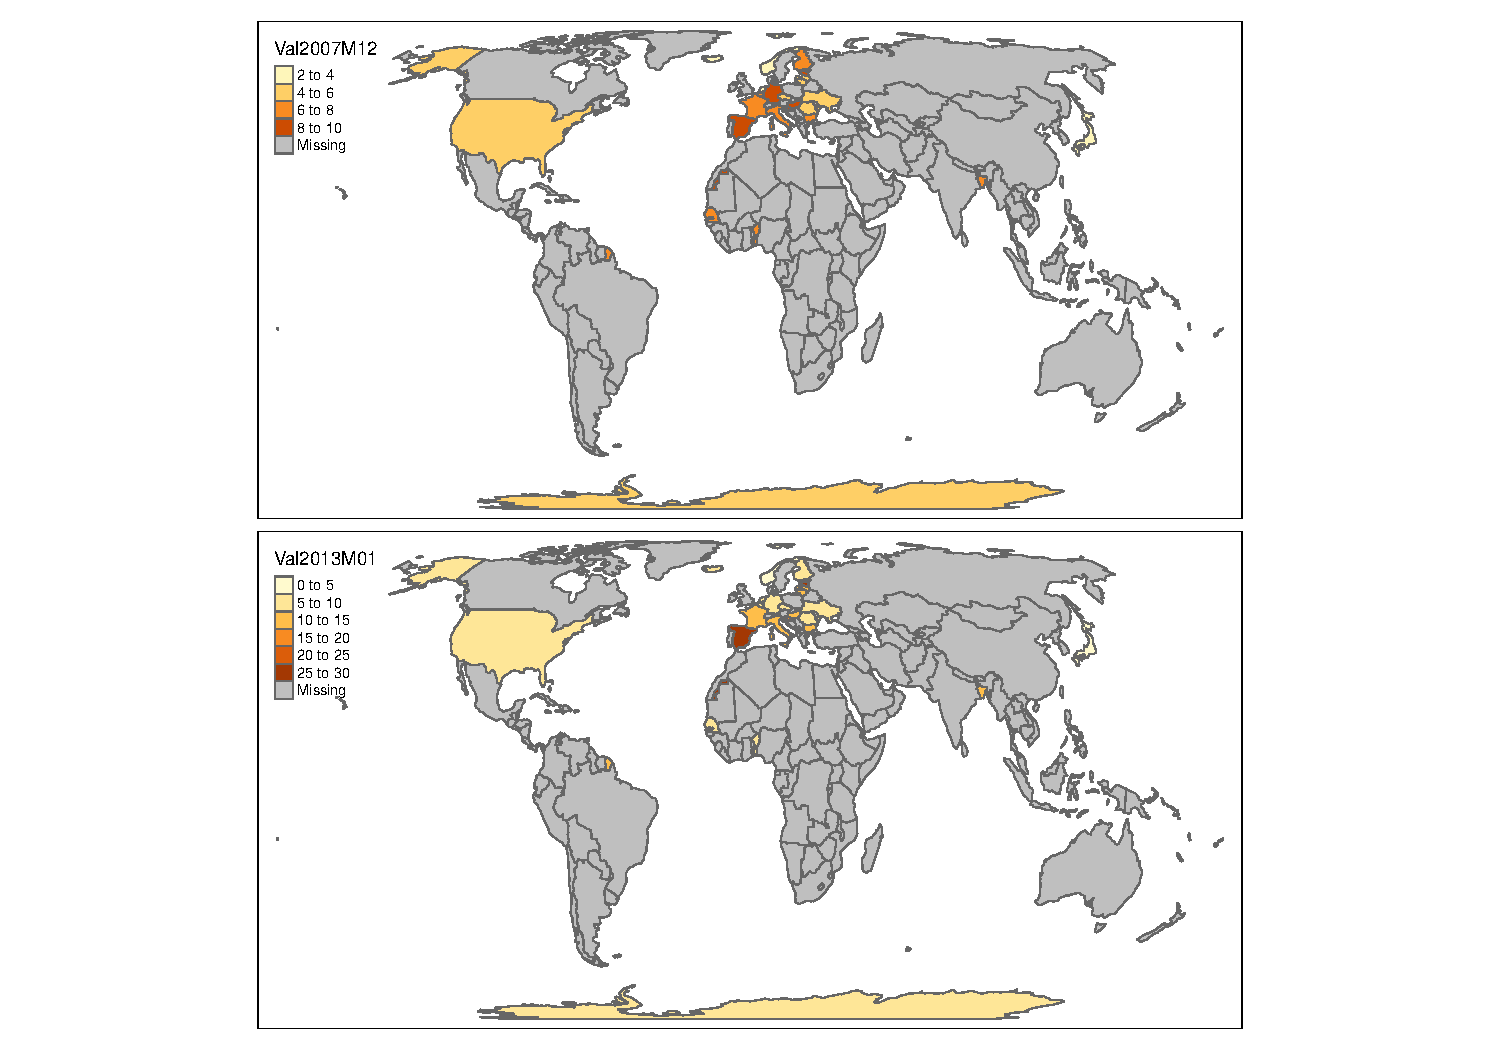
\includegraphics{quick_high_quality_maps_files/figure-beamer/unnamed-chunk-46-1.pdf}
\end{frame}

\begin{frame}[fragile]{}
\protect\hypertarget{section-1}{}
\begin{Shaded}
\begin{Highlighting}[]
\KeywordTok{library}\NormalTok{(}\StringTok{"choroplethrMaps"}\NormalTok{)}
\end{Highlighting}
\end{Shaded}
\end{frame}

\end{document}
